% REMEMBER: You must not plagiarise anything in your report. Be extremely careful.

\documentclass{l4proj}

    
%
% put any additional packages here
%
\usepackage{pdfpages}

\begin{document}

%==============================================================================
%% METADATA
\title{A Seamful Game Based on GPS Shadows}
\author{Robbert Malcolm Sinclair}
\date{24 March 2023}

\maketitle

%==============================================================================
%% ABSTRACT
\begin{abstract}
    The Global Positioning System, also known as GPS has revolutionised the way
    that we travel and position ourselves. While ideally we would want our GPS
    coordinates to be accurate, being around urban areas can obstruct the signals
    that allow for precise positioning. This project utilised the ideas of Seamful
    design to create a game which takes advantage of inaccuracies in GPS. The Gameplay
    was a simple game of tag in which players could use GPS shadow areas to hide
    from a chaser. After two user evaluations, I found that the reception of the game
    was positive although there were challenges due to the differences in devices in
    terms of GPS quality.  
\end{abstract}

%==============================================================================

% EDUCATION REUSE CONSENT FORM
% If you consent to your project being shown to future students for educational purposes
% then insert your name and the date below to  sign the education use form that appears in the front of the document. 
% You must explicitly give consent if you wish to do so.
% If you sign, your project may be included in the Hall of Fame if it scores particularly highly.
%
% Please note that you are under no obligation to sign 
% this declaration, but doing so would help future students.
%
\def\consentname {Robbert Malcolm Sinclair} % your full name
\def\consentdate {24 March 2023} % the date you agree
%
\educationalconsent


%==============================================================================
\tableofcontents

%==============================================================================
%% Notes on formatting
%==============================================================================
% The first page, abstract and table of contents are numbered using Roman numerals and are not
% included in the page count. 
%
% From now on pages are numbered
% using Arabic numerals. Therefore, immediately after the first call to \chapter we need the call
% \pagenumbering{arabic} and this should be called once only in the document. 
%
% Do not alter the bibliography style.
%
% The first Chapter should then be on page 1. You are allowed 40 pages for a 40 credit project and 30 pages for a 
% 20 credit report. This includes everything numbered in Arabic numerals (excluding front matter) up
% to but excluding the appendices and bibliography.
%
% You must not alter text size (it is currently 10pt) or alter margins or spacing.
%
%
%==================================================================================================================================
%
% IMPORTANT
% The chapter headings here are **suggestions**. You don't have to follow this model if
% it doesn't fit your project. Every project should have an introduction and conclusion,
% however. 
%
%==================================================================================================================================
\chapter{Introduction}

% reset page numbering. Don't remove this!
\pagenumbering{arabic} 


Why should the reader care about what are you doing and what are you actually doing?
\section{Guidance}

\textbf{Motivate} first, then state the general problem clearly. 

\section{Writing guidance}
\subsection{Who is the reader?}

This is the key question for any writing. Your reader:

\begin{itemize}
    \item
    is a trained computer scientist: \emph{don't explain basics}.
    \item
    has limited time: \emph{keep on topic}.
    \item
    has no idea why anyone would want to do this: \emph{motivate clearly}
    \item
    might not know \emph{anything} about your project in particular:
    \emph{explain your project}.
    \item
    but might know precise details and check them: \emph{be precise and
    strive for accuracy.}
    \item
    doesn't know or care about you: \emph{personal discussions are
    irrelevant}.
\end{itemize}

Remember, you will be marked by your supervisor and one or more members
of staff. You might also have your project read by a prize-awarding
committee or possibly a future employer. Bear that in mind.

\subsection{References and style guides}
There are many style guides on good English writing. You don't need to
read these, but they will improve how you write.

\begin{itemize}
    \item
    \emph{How to write a great research paper} \cite{Pey17} (\textbf{recommended}, even though you aren't writing a research paper)
    \item
    \emph{How to Write with Style} \cite{Von80}. Short and easy to read. Available online.
    \item
    \emph{Style: The Basics of Clarity and Grace} \cite{Wil09} A very popular modern English style guide.
    \item
    \emph{Politics and the English Language} \cite{Orw68}  A famous essay on effective, clear writing in English.
    \item
    \emph{The Elements of Style} \cite{StrWhi07} Outdated, and American, but a classic.
    \item
    \emph{The Sense of Style} \cite{Pin15} Excellent, though quite in-depth.
\end{itemize}

\subsubsection{Citation styles}

\begin{itemize}
\item If you are referring to a reference as a noun, then cite it as: ``\citet{Orw68} discusses the role of language in political thought.''
\item If you are referring implicitly to references, use: ``There are many good books on writing \citep{Orw68, Wil09, Pin15}.''
\end{itemize}

There is a complete guide on good citation practice by Peter Coxhead available here: \url{http://www.cs.bham.ac.uk/~pxc/refs/index.html}. 
If you are unsure about how to cite online sources, please see this guide: \url{https://student.unsw.edu.au/how-do-i-cite-electronic-sources}.

\subsection{Plagiarism warning}

\begin{highlight_title}{WARNING}
    
    If you include material from other sources without full and correct attribution, you are commiting plagiarism. The penalties for plagiarism are severe.
    Quote any included text and cite it correctly. Cite all images, figures, etc. clearly in the caption of the figure.
\end{highlight_title}


%==================================================================================================================================
\chapter{Background}
\label{background}

In this chapter I will go over some of the foundational concepts required to understnad the background of the project

\section{Introduction to the Global Positioning System (GPS)}

The Global Positioning System, also known as GPS, is one of the world's most famous Global Navigation Satellite Systems (GNSS). It allows people to determine their
location from anywhere around the world at any time. GPS has three main phases, the space phase, the control phase and the user phase.
In the space phase, the earth is split up into 24 "slots" which should be filled up by an operational satellite \citep{spsStandard}. Therefore
the GPS constellation is made up of at least 24 opterational satellites. In an ideal situation a user should have access to at least 4 of the satellites
at any one time \citep{Rabbany2006}. 

Each GPS satellite consistently sends down radio signals down to the Earth's surface. As of 2020 there are three main frequencies,
these are L1 which emits at 1575.42 MHz, L2 which emits radio waves at 1227.6 MHz and L5 with 1176.45 MHz \citep{spsStandard}. This project
will most likely be using L2 and L1 as L5 is used mainly for aviation safety \citep{Xu2016} A GPS receiver will pick up this data and can use the clock signals to calculate the distance from each satellite. Once a 
satellite distance is calculated we can create a radius of equidistant points. We can then add the signals from several other
satellites to find the intersection points. We usually need 3 to 4 satellites to be able to pinpoint the GPS receiver on the map. \citep{Rabbany2006}



%TODO - Add a source and paragraph about how GPS is calculated

\subsection{GPS in smartphones}
These days most smartphones are fitted with a GPS sensor to allow for precise navigation. However GPS is not the only GNSS
system that smartphones use. Multiple countries have launched their own satellite systems. For example Russia has the GLONASS
system, the European Union has the GALILEO system, China has the Beidou system. Most modern smartphones make use
of some or all of these systems. For example my personal phone and the phone that I am testing this project on, the Samsung 
Galaxy S21 FE makes use of all of the above mentioned GNSS systems \citep{samsungs21specs}. This means that in reality
a phone will be in sight of roughly 15 to 16 satellites rather than the usual 4. This means that phones can
have a lot more accuracy than in the past as the increase in satellites means that there is less chance of there being big
errors.

\section{What causes Inaccuracies in GPS Systems}
In this project we will be looking at making a game based on GPS shadows which are areas where the GPS signal is not as accurate. In this section I will look
at the various factors that could effect our accuracy.

\subsection{GPS Clock Errors}
% ROUGH DRAFT - Rewrite this with proper sources when you've found them

The first form of GPS error is a clock error. Each satellite sends signals down using an atomic clock which while accurate, can still have a 
slight delay. This delay will be small (a few nanoseconds long) but will accumulate over time. One of the main reasons why this can lead to
a decrease in accuracy is that the receiver may get a time on the clock which is off the actual time on the satellites clock. This can lead to
a slight change of position. This form of error is common with most GPS signals. A typical GPS Receiver can also be a cause for this problem as it 
has a crystal clock which is not as precise than the cesium atomic clocks on the satellites \citep{Rabbany2006, Kleusberg1990}. While this
form of error is a common cause of problem with GPS accuracy, there aren't a lot of game opportunities due to the fact that the player
can't really control when a clock error is to happen.

\subsection{GPS Signal Reception}
GPS signals are in the form of radio waves which can be blocked by obstacles on the way to a GPS sensor. When signals hit a specific obstable
the signals decrese in quality during a process known as attenuation \citep{Indoor2010}. Some examples of such obstacles include
building walls, soil and water. \citep{Kleusberg1990}. Eventually the GPS receiver will receive more noise
than the original signal which leads to an inaccurate signal. A good signal is received when the receiver has a good signal from at least 4
satellites. Therefore in urban areas with high rise buildings, one or more satellites could be obstructed. If a game was to be made
using this concept then the game would be best played in dense urban areas.

\subsection{Multipath Error}
Another factor which may affect the accuracy of a GPS error signal is a type of error called Multipath. This kind of error is particularily
common in urban areas. When a satellite signal goes towards a building, the signal will bounce of it and go into a different route to the
sensor rather than going in a direct route. As a result, the GPS coordinates may be considered to be further away than initially thought.
This is because the signal will take longer to find the sensor which means that the sensor will think that the true location is further than
initially thought.

Some ways to mitigate a multipath error is to go into a more open area or to have a different and improved design
of antenna \citep{Kos2010}. This means that if I were to make a multiplayer game, I may find that some phones are
more prone to having multipath problems than others. Another way to mitigate a multipath error is to use the 
satellite noise ratio to see how weak the signal is. When a GNSS sensor receives a signal, it is able to calculate 
the noise ratio to see how strong the signal is. You can then go over each satellite in turn in order to see how
good or bad the signal is. When the ratio is closer to 0 then you can say that it is likely that a satellite is blocked
while a ratio 1 would suggest that the satellite has a direct line of sight of the sensor \citep{uberGPS}. If I were
to make a game based on multipath I could give the user a label showing them the noise ratio and then see how the ratio
increases or decreases over time.

\section{Seamless and Seamful Design}
With most systems there will be potential seams which can cause unintended results to the user. One way to solve this would be to think seamlessly which is where you
try and fix every flaw so that your system is more robust. In the context of GPS, it is usually important to think seamlessly
so that people are able to easily to get to your destination. For example \cite{uberGPS} designed a system to improve their
GPS coordinates using 3D mapping and SNR noise ratio to ensure that Uber drivers were more likely to reach their customers. In this
case it was important to work seamlessly as Uber's business model relies on people getting from one place to the other, therefore it
is crucial for drivers to know that they are in the right place. In game design, seamless design is useful when there are significant balance issues. For example making sure to fix
glitches in order to prevent cheating. 

While trying to close every seam may be appropriate in some areas, it can sometimes be futile to try and close every seam.
Seamful design is the idea of embracing the seams in the system. In the context of GPS this usually means to try and embrace
the idea that GPS accuracy can vary based on the type of phone, the area you are in or the GPS clock error. For example 
\emph{Can you see me now?} a Mixed Reality game made by Blast Theory noted that while they were getting significant error radiuses they
were also finding that eventually the players were able to exploit the drops in GPS accuracy in order to catch other players. \citep{canyouseeme}

\section{Previous Work}

Over the years there has been several games that utilise GPS coordinates as a fundamental part of the game. In this section I go over two case
studies of location games that utilised seamful design.

One of the first location games was \emph{Can you see me now? (CYSMN)} which was a mixed reality made by blast theory. \citep{canyouseeme} The
game was played over a two day. There were three runners that would run around the streets of Sheffield
and Rotterdam. The goal of the runners were to catch players who were moving around in a virtual map. During the analysis of tactics displayed in the game,
\cite{canyouseeme} mentioned that the runners would have large ranges in GPS error which meant that some of the online players would get
caught without being able to see anything. Eventually the runners were able to take advantage of low GPS areas and were able to hide in shadow
areas.

\emph{Treasure} was a location based game created by \cite{Barkhuus2005} from the University of Glasgow. This was another GPS game which involved
collecting coins in a specific in a more open game area to ensure high GPS accuracy. The objective of the
game was to collect as many coins as possible, while also being able to "pickpocket" other players to steal their
coins. The pickpocketing worked by having a button that they pressed as they got close to another person. \cite{Barkhuus2005}
found that one of the big tactics that people would have is that they would take advantage of the lag in GPS coordinates
in order to pickpocket people from further away or to be able to get away from their victim quickly so they couldn't be
pickpocketed themselves.

Both \emph{Can you see me now?} and \emph{Treasure} found seams in their game design. In the case of CYSMN it was the accuracy
of the GPS coordinates, and in \emph{Treasure} it was the lag in GPS coordinates. While initially in both games they were seen
to be a flaw but as they got used to the mechanics, they were able to take advantage of them. For example there were several participants in 
CYSMN that stated that it was a "shame" that they were caught by a runner without seeing them. However when the runners embraced the inaccuracies,
it had increased the stakes of the game. \citep{canyouseeme}. We also saw that in \emph{Treasure} where the players took 
advantage in the lag between location updates to get away from their victims. When you expose seams to people, there can
be interesting ways that people exploit those seams to gain an advantage.

%==================================================================================================================================
\chapter{Analysis}
In this section I go over the main process that I used to come up with a design for the game

\section{Initial GPS Experiments}
\begin{figure}
    \centering
    \includegraphics[width=0.75\linewidth]{images/original_web.png}
    \caption{A screenshot of the original web application containing GPS shadow areas}
    \label{fig:analysismap}
\end{figure}
I started my analysis by learning the basics of learning app development by creating an app that would keep track
of GPS accuracy. The app started off as just a screen with my latitude and longitude coordinates and my error rates.
Once I had this app up and running, I walked around various locations around the University of Glasgow campus and
also briefley within the city centre. Some particular areas that I tried included more open areas like the Botanical
Gardens and Kelvingrove park and the area surrounding the main building including the cloisters. I also wanted to test
out the effect of standing next to tall buildings. To do this I tried standing really close to the Boyd Orr building
the tower of the main building to see if there were any significant decreases in accuracy.

During the experiment, I made a basic web server where I could send my coordinates and accuracy data to. From
there I put the locations on a map, a screenshot of which is shown in figure \ref{fig:analysismap}. I mapped
out the locations by sending data to the server whenever a new location was recorded. I then increased the spots
on the maps based on their error radius. The bigger the error radius, the bigger the circle on the map. This was
really helpful in understanding where GPS signals were most likely to decrease or increase in accuracy.

\section{Testing GPS APIs}
One of the other reasons for carrying out these experiments was to test out two Geolocation APIs. These
were the \emph{FusedLocationProvider} API and the \emph{LocationManager} API. In order to put these two
APIs to the test, I decided to take repeat the experiment with each API to look at the various ranges in
accuracy.

\subsection{FusedLocationProvider API}
\label{fusedProvider}
The first API I tried was the FusedLocationProvider API as this was the first one that I found. The FusedLocationProvider API combines both GPS and WiFi geolocation
techniques to try and create an optimal location \citep{fused}. This API allowed me to create a basic location app quickly so that I could start finding GPS locations
within my local area. As figure \ref{fig:fusedhist} shows, the location data that I gathered was skewed towards values with an accuracy of less than 50 metres. While a lot of
points were under the 20 metres area. However as you can see, there was a decent amount of values above 50 meters meaning that the API picked up a lot of shadows.
This API would have been a good one to use for my game as I would have had a lot of shadow areas for a player to hide. However the main flaw was that
it was giving me a combination of both Wifi and GPS coordinates. Thies meant that I was more likely to find shadows in areas with low WiFi. This would
explain why I had a lot of shadow areas when I walked around Kelvingrove Park, an area which I thought would have a very accurate signal due to the lack of buildings.

\begin{figure}
    \label{fig:phase2_ui}
    \centering
    \begin{subfigure}[b]{0.45\textwidth}
        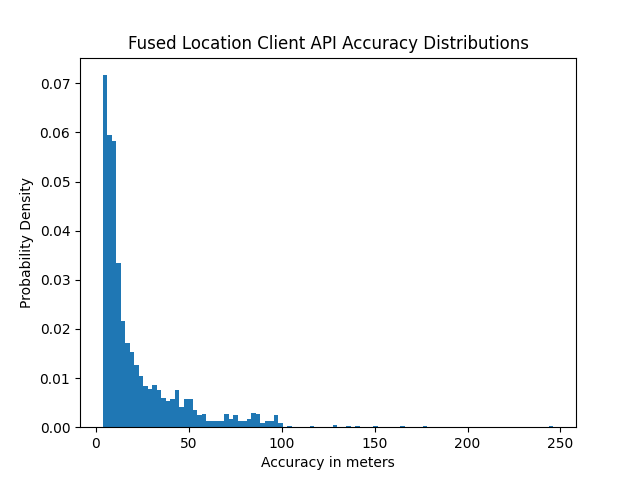
\includegraphics[width=\textwidth]{images/fused_histogram.png}
        \caption{Fused Location API}
        \label{fig:fusedhist}
    \end{subfigure}
    ~ %add desired spacing between images, e. g. ~, \quad, \qquad, \hfill etc. 
      %(or a blank line to force the subfigure onto a new line)
    \begin{subfigure}[b]{0.45\textwidth}
        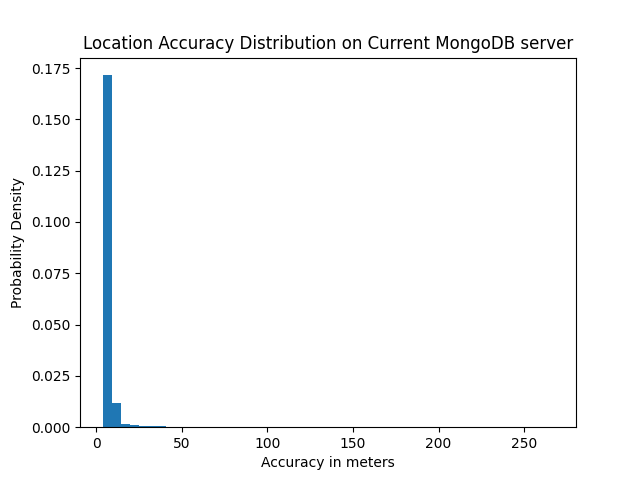
\includegraphics[width=\textwidth]{images/mongo_db_histogram.png}
        \caption{Location Manager}
        \label{fig:mongohist}
    \end{subfigure}
    
    \caption{These histograms show the ranges in accuracy between the Fused Location API and the
    Location Manager API
    }
\end{figure}

\subsection{LocationManager API}
\label{locationManager}
The second API that I tested was the \emph{LocationManager} API. This API gives me more control over what kind of Geolocation I was getting on my phone. Therefore
I was able to ensure that my geolocation was based on a full GNSS navigation system. \citep{locationManager} The other main advantage to this library is that with the use of the "requestLocationUpdates" method and
the "LocationListener" interface, I can easily control what my app does when it receives a new location. This API also allowed me to control the delay between location updates and the minimum
distance that a user will need to move before the location updates. This will be especially useful if I were to have features which were
more computationally demanding.

While there are some advantages to using the LocationManager API, it does come with some disadvantages as well. For one thing, there are significantly less shadow areas when using
pure GNSS coordinates. The only real areas where there are major shadows are within buildings, under bridges or in enclosed areas. This is because on my phone, it can track up to 
15 satellites when getting my location. In comparison to figure \ref{fig:fusedhist}, figure \ref{fig:mongohist} shows that there is one big peak in the overall accuracy of all the spots.
When walking around with my app I noticed that for most of the time, my accuracy was 3.795 meters of accuracy. However while at first glance this may be a disadvantage the main advantage for creating a
game is that compared to the Fused Location API. It is better overall for an overall game design because the areas where shadows can be found will be more consistent than the ones
found in the Fused Location API. Therefore the game can be used to teach people where GPS can decrease in quality.

\section{Conclusions from the location experiment}
After reviewing the data from both the \emph{FusedLocationProvider} API and the \emph{LocationManger} API,
I decided that I would use the LocationManager API for Geolocation. While it had less shadow areas than
the Fused API, the purely satellite based positioning meant that the shadow areas were more consistent overall.
With the LocationManager API the shadow areas were in more obvious areas that an ordinary person would think
about when trying to decrease their signal quality. The \emph{FusedLocationProvider} on the other hand
would have shadow areas where there wasn't good WiFi signal despite there being good satellite signal.
This led to the discrepencies in accuracy within Kelvingrove park for example.

While my primary objective was to find the best Geolocation API for creating a game, I also wanted to 
know where I could set a game that would have a balance between shadowy areas and more open areas. From
the data that I have I knew that the game would have to be played in a built up area. While I expected
fields in a park to have high GPS accuracy, I was surprised that going into a forested area didn't affect
the accuracy much either. I found that the best results for decreasing your GPS accuracy was to stand
under bridges or to go inside buildings. Using this information, I decided to pick the main building
of Glasgow University. The main reason for this was that I found lots of shadows in that area. I figured
that players had a lot of places to hide like the cloisters or the University chapel. I also felt that
the area was small enough to keep the game exciting for shorter games.

%==================================================================================================================================
\chapter{Phase 1 Design}

\section{Process}
\label{phase1designprocess}
Once I got a rough understanding of how GPS works, I then decided to have a think about what kind of games I could make
with the information I had considered. I started by having a general brainstorm of what kinds of games I could adapt.
These ideas ranged from simple games like Tag games such as \emph{Manhunt} or \emph{Stuck in the Mud} to several wide
games that I played in primary school. One notable idea was a game where people with a GPS sensor have to travel to a
destination without being visible on the map. If they are visible, a watcher would be able to tap on their marker. If
that happens the GPS players would have to go back to the start. I found that this idea didn't work after making the
move to the LocationManager API (See section \ref{locationManager} for more details) since the amount of high accuracy
areas greatly outnumbered the shadow areas.

Once I had completed my brainstorm, I took the ideas that would be feasible to do and started to expand on the ideas a
bit more. To do this I took a piece of A4 paper, and filled it with ideas of particular Game Mechanics. This allowed me
to form ideas of what kinds of games would be fun to play. Figure \ref{fig:idea1} shows an example of one of these sheets.
As you can see they are rather rough but this exercise let me formulate the mechanics, the aims and the winning conditions.
Also by drawing diagrams, I got better ideas of what the user interface would look like.

After going through those two processes, I took one idea and started generating wireframes using Figma. At this point I
looked at the technical requirements to get the game working. This usually involved researching what technologies to
use and to start experimenting with them.

\begin{figure}
    \centering
    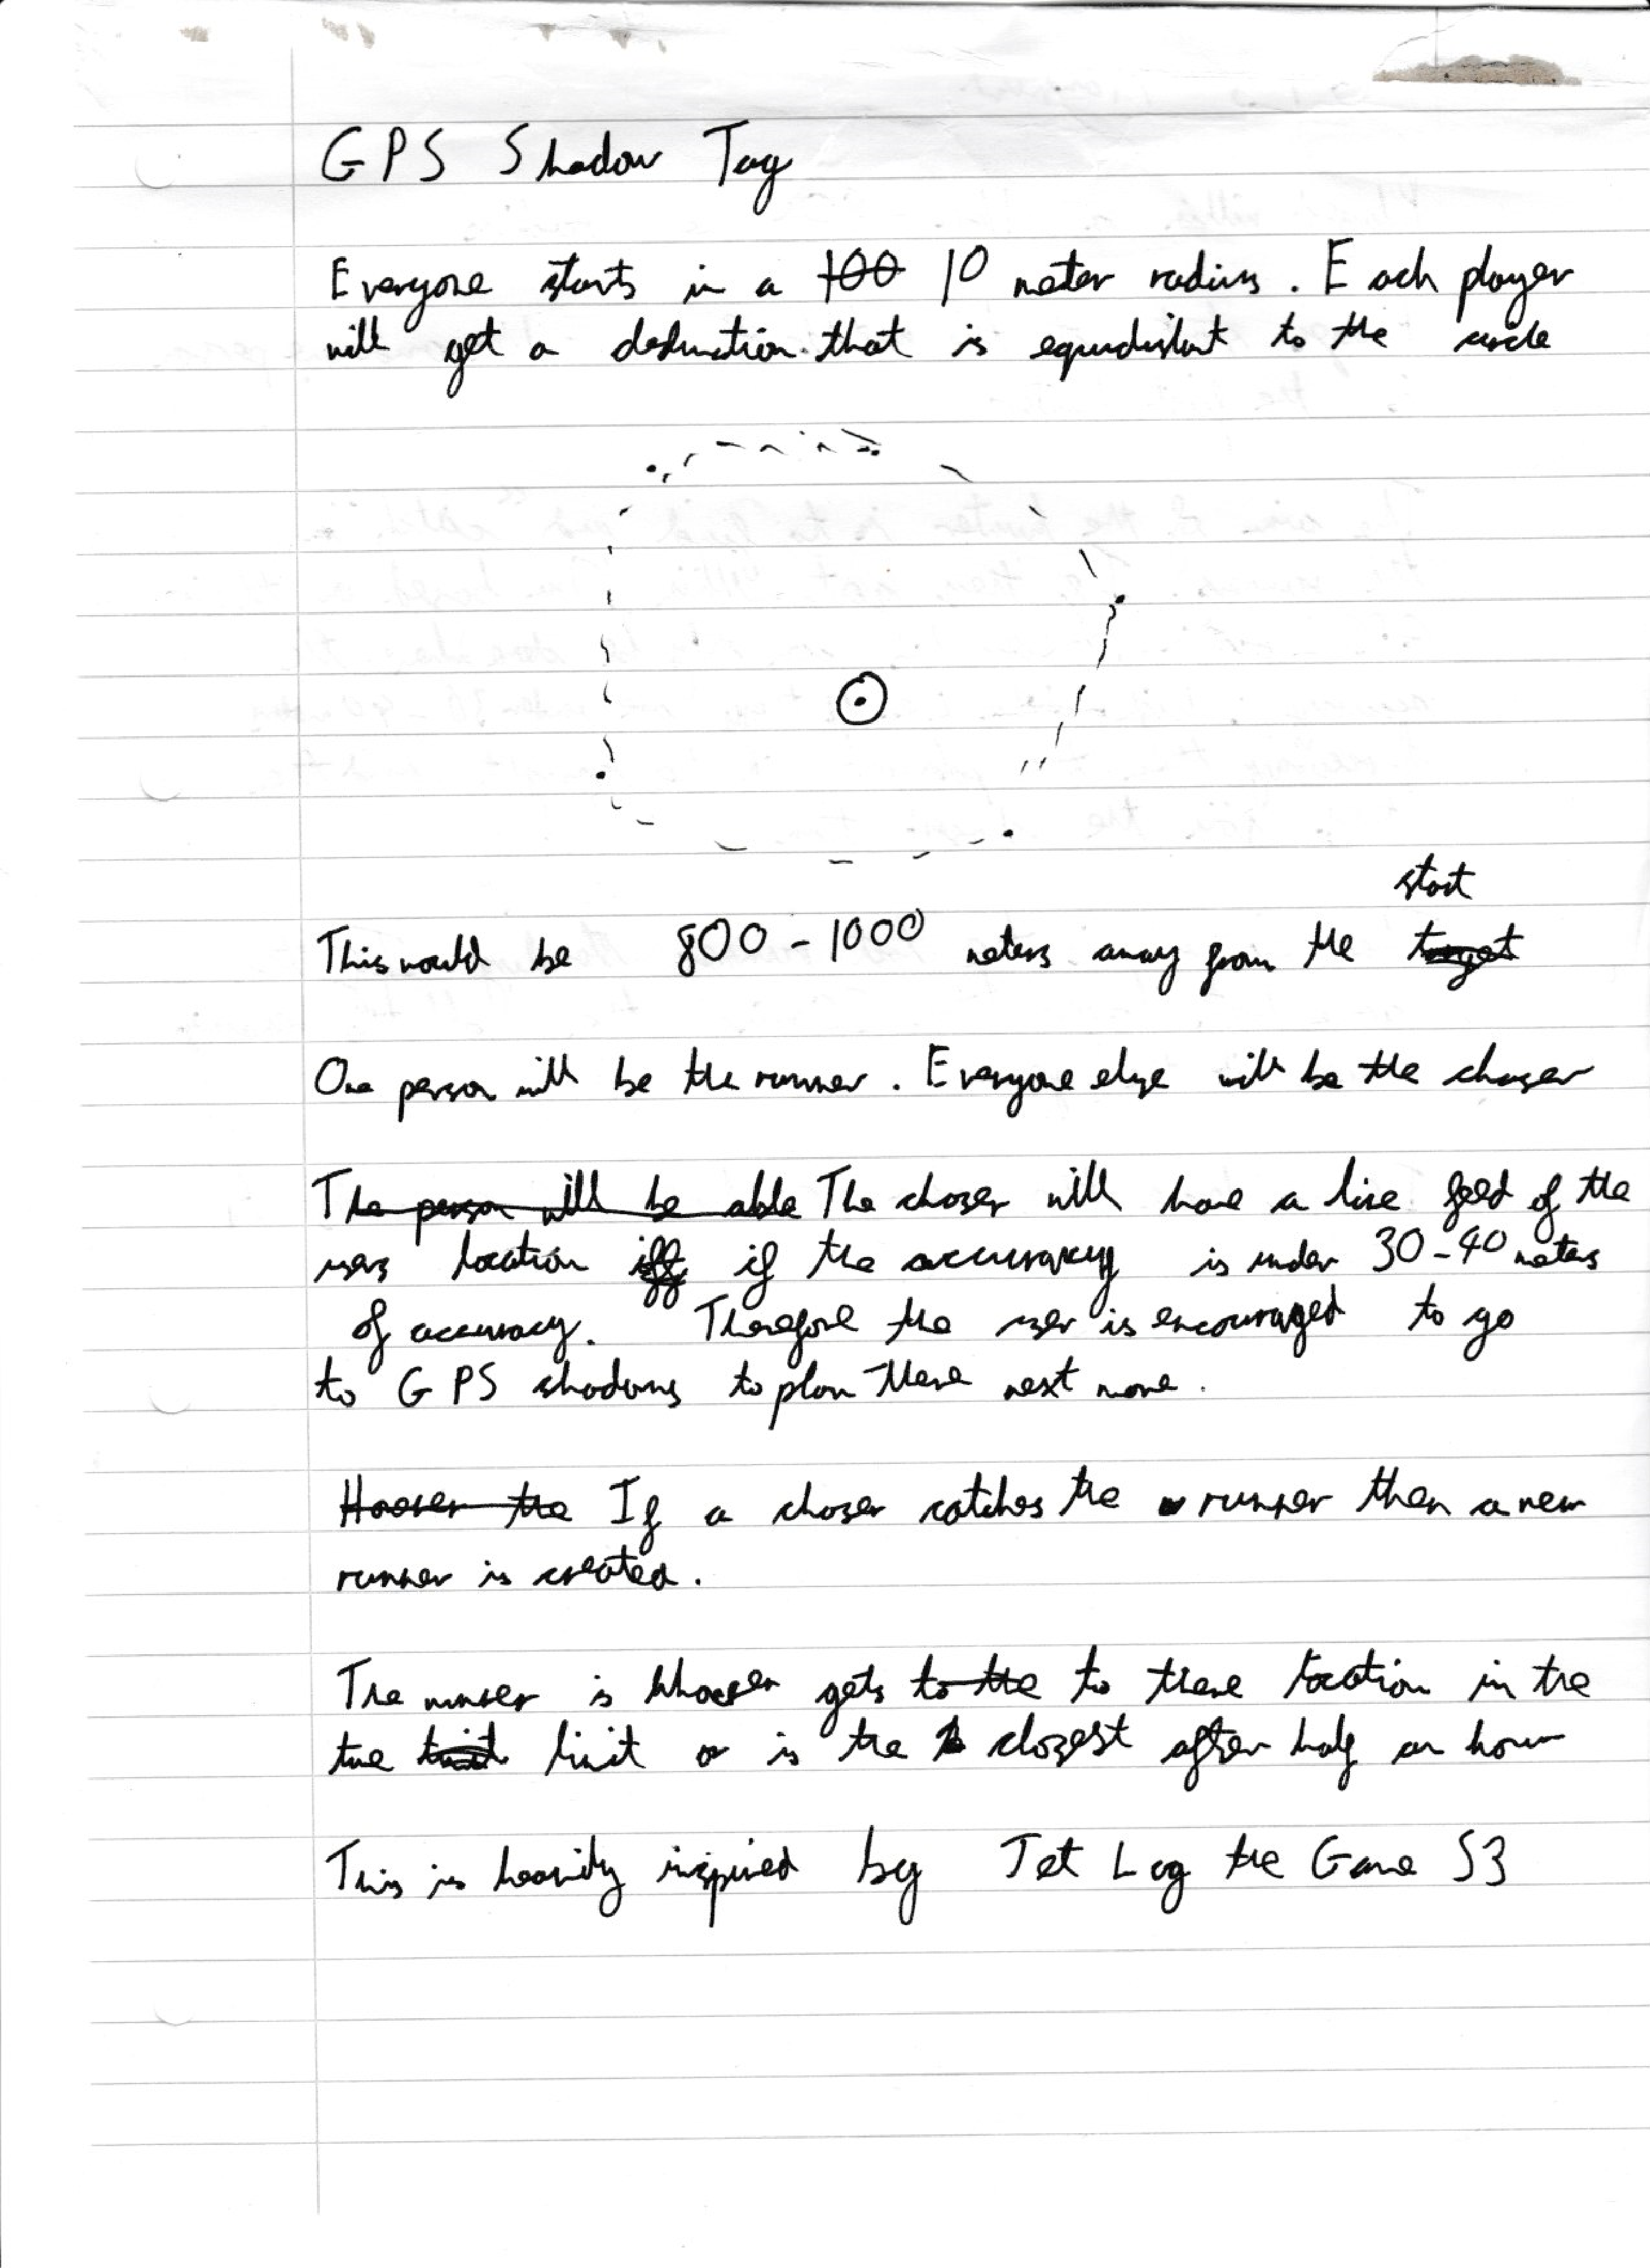
\includegraphics[width=0.5\linewidth]{images/idea1.pdf} 
    \caption{My rough paper draft of idea 1}
    \label{fig:idea1}
\end{figure}

\section{Overview}
\label{game-overview}
After going through all of the steps described in section \ref{phase1designprocess}, the game idea that I settled On
was a simple tag game where a player can take advantage of GPS shadows in order to hide from
a "chaser" player. The chaser will be able to see the other users locations in real time if the runner is in an area with
high GPS accuracy. Once a chaser tags a runner, the caught runner becomes the chaser and a 30 second Jail Time is
triggered. During this time the catcher cannot see the runner's latest location or is able to catch a runner.

The game will have a time limit with the first iteration being 15 minutes. This is so that the game can be quick and
easy to play during a study break. I also considered the fact that the game would work well in dense urban environments
with lots of buildings to go into like the University of Glasgow campus. Once the time limit is up, the winner will
be calculated as the person who was the runner for the most amount of time in total.

\section{Architecture}
\label{phase1architecture}
The game that I will create will utilise a Client-Server Architecture. The client will be a smartphone with a GPS or
GNSS sensor. Several clients will be connected using a WebSocket. The smartphone will get the GPS data including the
latitude, longitude and accuracy and then will process it and send to the server. The location data will also be sent 
to the UI where the user's overall position will be updated. Through the websocket, the phone will send the GPS data
to the server which will save the users location onto a geospatial database. Depending on certain conditions, the data
will be sent to the rest of the clients.

Since the clients of the game will be smartphones. I decided that the game will take a thin-client design with the
server handling most of the game logic. This is due to the range of computational abilities of different phones. 
I feel that a server will be able to handle lots more computations over time compared to the average smartphone.
It also means that it is easier to keep track of who is the chaser, who has been caught and where they are on the map.
There will still be some features that will be implemented on the client, this includes a timer and the calculation of
jail time. However to ensure that no player has an unfair disadvantage, I will keep track of the game time on the
server as well. This is so that we can keep the game in sync with other players.

\subsection{Client (Smartphone)}
\label{designClient}
The smartphone app will be divided into four main components. These are the GPS Listener, the Communications area, the
Player and the User Interface. When the client first connects to the server, it will give the user a player id and a player
type. This information will be given to the player class which stores the id for any further communications with the server.
Then once that is done, the GPS Listener will start to fetch the GPS coordinates every 2 seconds. This data is then sent
to the User Interface so that the map is updated with the user's location. The GPS coordinates are then sent to the Communication
class where they are sent to the server.

\subsection{Client Server Communication}
\label{communication}
Since a lot of the game will have a lot of multiplayer features, it was important that the network side of the game
was robust to ensure that no player would have an unfair advantage when playing the game. Some examples of messages that the server
could give the user includes:

\subsubsection{CONNECT}
This message connects the user to the server. The server will then send over a user id.

\subsubsection{NEW\_TYPE}
This is triggered if either a new user connects to the server or if a user is caught. The server will keep track of what
type of player the person .

\subsubsection{PLAYER\_CAUGHT}
\section{Mechanics}
In this section I go over the various mechanics that I have designed for the game

\subsection{Player Types}
When the player joins the game, they will be assigned to one of two player types. These are the "Chaser" or the "Runner".
The role of the Chaser is to catch a runner as described in section \ref{catching}. When the catcher does this they give the role of chaser to the runner. The Chaser
will be able to see the real time locations of any runner in the game.

The goal of a Runner is to avoid being caught by the Chaser as mentioned before. The Runner will not have a real time
view of the Chaser but will have the ability to "hide" from them by going into areas with a low GPS density. If their
GPS accuracy is low enough, they will not transmit their location to the chaser. Making them invisible to the chaser.
The Runners will also not transmit any location data during the jail period as mentioned in section \ref{game-overview}.

In previous iterations of my design the Runner would have been able to have seen all of the GPS Shadows within a 50
metre radius. The Shadows would be small red dots on the users maps. However after implementing this feature the screen
would freeze up leading to a poor user experience and it gave the Chaser an unfair advantage as they didn't get any
performance issues with just the Runner locations on the screen.

\subsection{Location Tracking and Catching}
\label{catching}
As mentioned before, both the runner and the chaser transmit data to the server. After a set interval
the latest latitude and longitude coordinates will be sent to the server which will update the player's location
in the database. Once this data is collected the chaser is then able to determine if they have caught a runner.

The chaser will have a 5 meter "no-go zone" which will be the way to determine if a player is caught or not. If
the GPS accuracy is high and a player has entered the Chaser's 5 meter radius, then the runner is considered to be 
"caught". In order to encourage players to look for shadow areas, for this phase a catcher will not be able to catch
a runner if they are beyond the 6 meter catching radius. Overall I felt that using a 5 metres was a good radius to 
start with. This is because 5 meters should be enough to account for multipath errors and that it would be close enough
for a runner to recognise that they are caught.

\subsection{Jail Time}
When a runner is caught, as the new chaser they will be put in Jail Time for 30 seconds. The main reason for this is
to give the new runners a head start to get out of the area. During this time, the chaser will still be able to move
around, but they won't have a view of the runners location nor can they catch them. The runner will also get a message
that the chaser is in jail time. I decided on 30 seconds because in most urban areas, it is enough time to get out of
eyesight from the chaser. I also knew that I needed to strike a balance between giving the runners enough time to get
away but at the same time not being so much time that there is not enough time for the chaser to catch the runner. 

\subsection{Time Limit and Winning Condition}
From the start I felt that I needed to consider how long a game should last. I wanted the game to be fast and fun to
play in a short amount of time since I was aiming at university students. Therefore for this phase of design, I decided
on 15 minutes. The main reasons why I picked this time is because it would be too long to go a really long distance.
This means that both the chaser and the runner will be within a very small area. My hope is that this will lead to
a greater frequency of catches during the course of the game.

For this phase of development, I wanted to keep the winning condition simple. Since I wanted to focus on defining the
main mechanics of the game, I didn't have a lot of time to think about the condition in which a player could win the
game. Therefore I decided to keep things simple by saying that the winning player would be the one who spent the longest
time as a runner player. I felt that since the core mechanic of this game is to keep out of sight from the chaser, if you
lasted a long time without being caught, then there is a chance that you found a good way of keeping hidden.

\begin{figure}
    \centering
    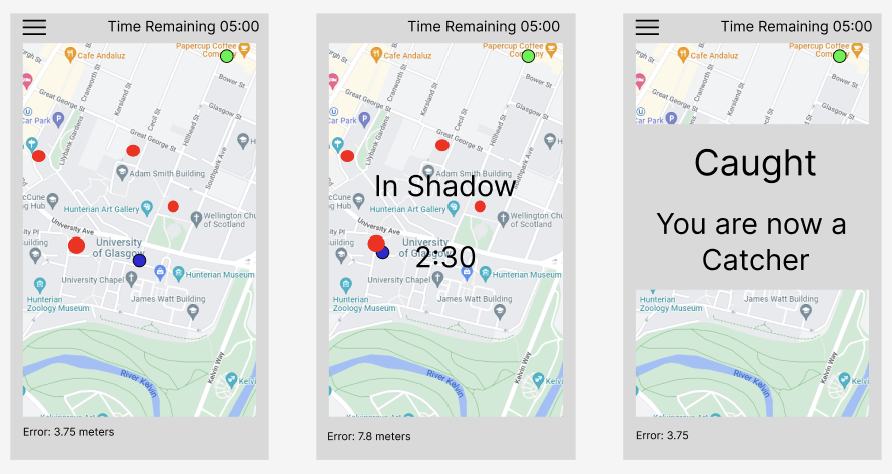
\includegraphics[width=0.7\linewidth]{images/phase1UIDesign.png}
    \caption{One of the figma wireframes that I created during my UI design. The first wireframe shows the overall view that a runner
    player will see, the second frame being what the runner sees when they are in a GPS shadow and the final frame being the view when
    the player is caught.}
    \label{fig:phase1uidesign}
\end{figure}

\section{User Interface}
\label{phase1uidesign}
Once I had designed the main mechanics of the game, I wanted to make a design of the User Interface. To do this I created a wireframe
on Figma to generate an overall wireframe. Figure \ref{fig:phase1uidesign} shows my initial designs for this phase of the game. Since
this is going to be a location based game, I knew that it would be important to have a map in the centre of the screen. In the first
wireframe, I show the overall view that a runner player would be able to see. In this case the blue dot shows you the runners location while
the red dots show the locations of the various shadow areas that I found during my analysis phase. My hope is that this would give the
users an idea of what areas would be good to hide in.

The second and third frames in \ref{fig:phase1uidesign} show what happens when the runner is in a shadow and whenever the runner has been
caught. The plan would be that in the third frame, it will include several differnt messages like whether a player has joined or left the
game, to inform the player that the game has ended or to inform the player on what player type they are. 




%==================================================================================================================================
\chapter{Phase 1 Implementation}
\label{phase1implementation}

\section{Process}
\label{process}
The game was developed using an iterative approach where I took the time to design some game mechanics, implement them and
then evaluate it with other users. This has helped me when designing the core mechanics of the game and it has allowed me
to see what other people would want in future iterations.

\section{Technologies Used}

\subsection{Server}
\label{implementationServer}
When designing my system, I knew early on that I needed to set up a server in order to keep track of people's location
and to give the user updates on who is playing or not. To do this I needed a server side framework that would make real
time communication easier and that would allow me to easily implement a WebSocket. Initially I made a Django server to
handle the requests making use of the Django Channels library. However this proved difficult when deploying the application.
This was because in order to use Django with a WebSocket you need to configure it with ASGI rather than the default WSGI
to allow for asynchronous communication. This proved to be rather difficult, therefore I decided to abandon Django for this
project.

The final version of the server is written using Node.js. The main reason why I decided to migrate to this technology is that
I could easily set up what I needed without worrying about all of the extra stuff that I would need to implement if I where to
stick to Django. It also had an easier WebSocket library \emph{ws} which allowed me to develop my communication system quickly
and effectively. Another benefit to using Node.js was that I could use any database that I wanted meaning that I could
choose the right one for the job. If I were to have stayed with Django I would have been limited to popular SQL databases
such as PostGreSql, Oracle or MySQL \citep{djangoDatabases}. Node.js allows me to be more flexible and it's light weight
design means that I can make the server side code as big or as small as I need it to be.

\subsection{Database}
\label{implementationDatabase}
As I mentioned in section \ref{implementationServer}, the freedom of using Node.js meant that I could really have a look
around for suitable databases. Since the design of the catching mechanic was that the chaser had a no-go radius (see section
\ref{catching} for more details), I decided that I wanted to use a database which had the potential to have Geospatial queries.
Two of the most popular databases that would allow me to do that would be PostGIS which is a modified version of PostGreSql \citep{postgis, postgres} and
MongoDB which is a popular document based database \citep{mongodb}. In the end I decided to go with MongoDB since their API
was easy to use and integrate into my server design. With MongoDB I could use their GeoSpatial Processing with minimal setup. Also it is significantly
faster than PostGIS in processing proximity queries \citep{Bartoszewski2019}. This was especially important considering
that I would be querying this database every time another player broadcasts their location.

\subsection{Mobile App}
As mentioned in section \ref{designClient}, the client will interact with the game through a mobile app. After a lengthy
analysis of different programming languages and frameworks that I could use, I finally settled on making a native Android
app using the Kotlin programming language \citep{kotlin}. I chose to write my code in Koltin because it has a simple syntax
and is now the recommended language for building android apps by Google. It also contains UI libraries such as Jetpack Compose 
which makes UI design and implementation easy to implement.

Another main reason why I went for Koltin is that other cross-platform mobile frameworks did not have the APIs required
to get pure GNSS coordinates. Kotlin has the LocationManager API (See section \ref{locationManager}) which allows me
to gain GNSS coordinates and some vital information like the signal noise ratio (SNR) of each satellite \citep{locationManager}
which gives me a lot of further information which can be useful for creating algorithms that can determine whether a player
is in a GPS Shadow or not.

\subsection{Deployment}
\label{deployment}
Having the front-end of the game as a Kotlin app brought a couple of challenges when developing. For one thing, it meant
that I couldn't run my server locally if I wanted to test my location tracking or other features with my mobile app. Therefore
I needed to find a hosting service that would allow me to deploy quickly and with very little effort. Railway.app \citep{railway}
is a cloud base deployment service that auto deploys after every git commit. Since I had a GitHub repository, it meant that it was
easy to deploy my code onto a server. Therefore I could focus more on the overall development rather than how to get it on a server.

\section{Mobile Side}

\subsection{User Interface}
\label{implementationui}

\begin{figure}
    \label{fig:ui_imp}
    \centering
    \begin{subfigure}[b]{0.25\textwidth}
        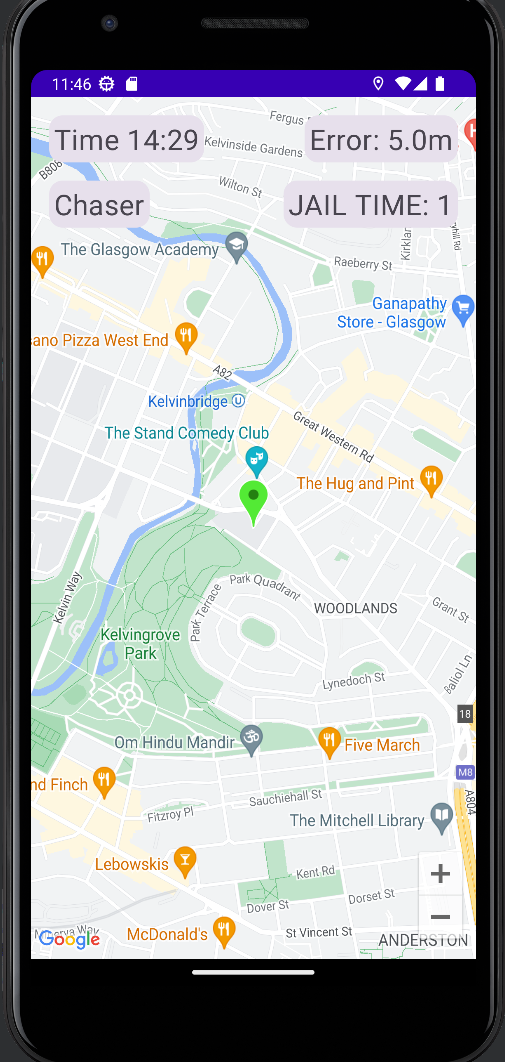
\includegraphics[width=\textwidth]{images/ui_chaser.png}
        \caption{The Chaser view.}
        \label{fig:phase1_ui_chaser}
    \end{subfigure}
    ~ %add desired spacing between images, e. g. ~, \quad, \qquad, \hfill etc. 
      %(or a blank line to force the subfigure onto a new line)
    \begin{subfigure}[b]{0.25\textwidth}
        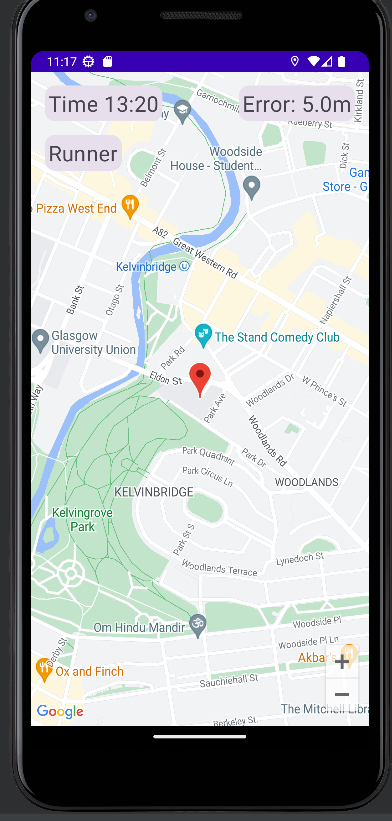
\includegraphics[width=\textwidth]{images/ui_runner.png}
        \caption{The Runner View}
        \label{fig:phase1_ui_runner}
    \end{subfigure}
    
    \caption{These two screenshots show the runner and the chaser states that the players
    will see when playing the game. \ref{fig:phase1_ui_chaser} shows you what a chaser player would
    see while the game is in progress while \ref{fig:phase1_ui_runner} shows you what a runner would
    be able to see.
    }
\end{figure}
For the game to be accessible to users I needed to make a User Interface that was
clear and simple to use for the duration of the game. Figures \ref{fig:phase1_ui_chaser} and \ref{fig:phase1_ui_runner} 
gives you a view of the two different screens that the player would get when they start a
game. The final design takes advantage of the Google Maps SDK for Android which has
an easy to use API for working with maps with Jetpack Compose \citep{GoogleMaps}.

The UI features at the top of the app are the same for both player types. On the top
left corner, the player has a view of how long they have left in the game, the timer
counts down from 15 minutes and is synced with the server time every 30 seconds to 
ensure that every player has the correct time. The top right of the UI gives the
user's GNSS error to 1 decimal places. This will give the user feedback on whether
their location is a good hiding spot or not. Finally the last row includes a label
to tell the player what type of player. To the right of that label is the "Jail Time"
label which only shows in the 30 seconds after a player is caught or when the game is
started.

As seen in figure \ref{fig:phase1_ui_chaser}, the Chaser view doesn't have a lot of extra features
compared to the runner view. The only main difference is that there is a marker to show the
runners locations. In both player types, the player's current location is marked in green and
all other players will have a red marker. This is in response to feedback from phase 1 (see section
\ref{phase1survey} for more discussion on this) as in that phase I had markers which were the same
colour.

The phase 1 version of the user interface has some differences when compared to the design in figure \ref{fig:phase1uidesign}.
The main difference being that there are no shadow markers on the runner map. While it was trivial to get some GPS shadows on
the server side, I found that when I tried to implement it on the mobile app, the amount of markers made the UI freeze up which
would have given the chaser an unfair disadvantage. The other differences was that I didn't implement the "in shadow" label,
I thought that since I moved my error label to the top of the screen, the player would be able to tell whether they were
in a shadow area by looking at the differences in their error radius as they move around. I felt that this would be better in
getting the player to understand where they would be able to find GPS shadow spots.

\subsection{LocationWebSocket}
During the course of my development, I had to create many different Kotlin classes in order for my front end to work properly.
One of the most important classes that I used was the LocationWebSocket class. The main purpose of this class is to set up a
real time connection with the Server and to control the different UI components that directly rely on server-side communication.
One of the big examples of this is the notification component. Whenever the server sends a message to the user, there will almost
always be a "message" key which will store a string to display to the user. When the LocationWebSocket class receives a message, it 
will start by getting the message and then it will display the message to the screen for 2 seconds.

As the name suggests, the LocationWebSocket is also responsible in ensuring that the mobile app has a consistent connection to the
WebSocket. When developing my first true iteration of the game, I would notice that after 5 minutes of game time, 
the app would disconnect giving me a "Failed" error (Please see section \ref{mongocollections} for more details on how I solved this problem on the server side). 
Luckily the library that I used to handle WebSockets, the OkHttp client \citep{okhttp} has a useful
interface which would allow me to implement an "onFailure" method. This meant that I could easily write some code that would automatically
reconnect the user, should their connection fail for whatever reason. Since I also had a class for storing the player's
details, I would be able to send to the server my player id so that the server would treat the new connection as if it was
the same player.

Overall the LocationWebSocket class gives the Mobile app all of the methods required to ensure that it is connected to the game
server and to ensure that the apps react to WebSocket messages effectively. While the two examples may have been useful. The most
important method, the "onMessage" function deserves its own section. In section \ref{websocketactions}, I will go over the mechanism
that I had in place to handle the different types of message that the server will give the Application.

\subsection{WebSocketActions}
\label{websocketactions}

\begin{figure}
    \centering
    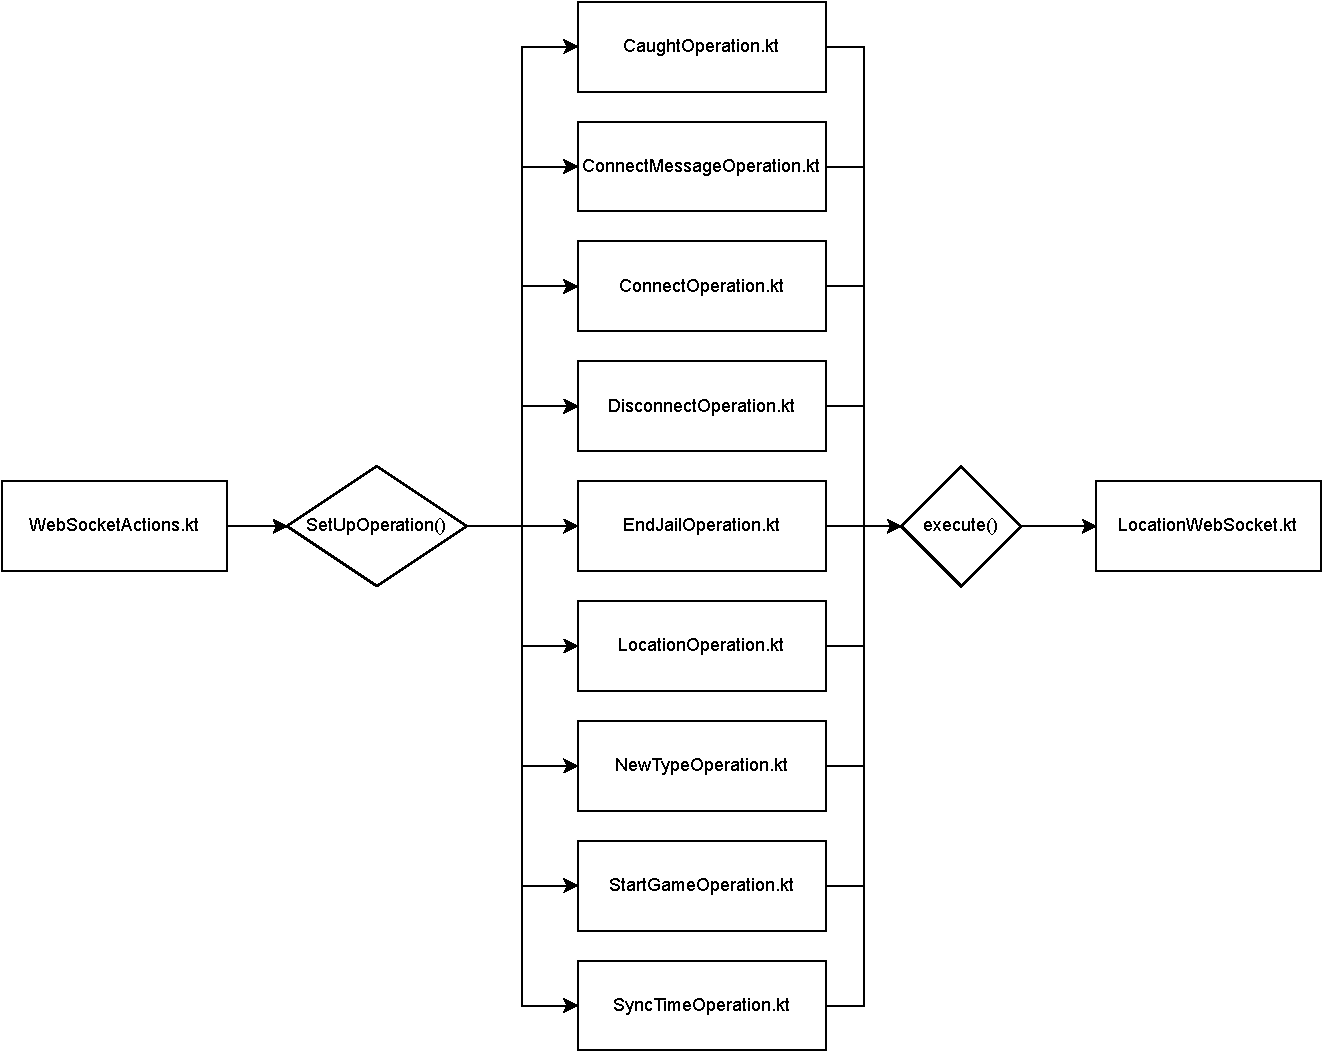
\includegraphics[width=\linewidth]{images/LocationActionsEnumDiagram.pdf}    

    \caption{
        This diagram shows the main architecture for the WebSocketActions enumeration. When a
        Websocket message is received by the application, the LocationWebSocket class will then
        read the type from the message JSON object. This will then create an instance of a specific
        operation class which all have an execute method.   
    }

    % use the notation fig:name to cross reference a figure
    \label{fig:locationActions} 
\end{figure}

The "onMessage" method of the LocationWebSocket class is probably one of the most important parts of the game.
One of the big challenges with both my design and development was working out how I was going to handle the multiple
different types of messages received from the server. Initially I had a conditional statement when I was first
testing out a connection to a WebSocket. However, I soon noticed that as the amount of operations increased, it
was going to get a lot harder to maintain my code if I kept going down that route. Therefore I decided to create
a new enumeration class called "WebSocketActions".

The WebSocketActions enumeration class acts as a bridge between the LocationWebSocket class and several similarly
structured classes that inherit features from a WebSocketOperation class. As figure \ref{fig:locationActions} shows, 
whenever there is a message from the server, the type of the message is used to tell the actions class which operation
class to build. Once the class has been found, we can then run an "execute" method to execute the operation that had
to be done on each message.

One of the most notable and important action that I have implemented is the LocationOperator. This is run when the player
is the current chaser on the map. If the server registers that it is under the shadow threshold, it sends over the
players location. When this message happens, an instance of LocationOperation is created and when it executes, it
takes the coordinates of the other player and creates a Google Maps class which allows me to place a marker on the
screen. Since this message is sent often, the chaser is able to see an almost real time view of where the other players
are if they are in a high signal area.

Another important operation in the WebSocketActions enum is the NewTypeOperation, this happens when the player has received
a NEW\_TYPE operaiton. This typically happens when the player is caught by the chaser or if the current chaser disconnects.
When this operation is executed, the player is informed of what new player type has been created. Then it starts the "Jail Time" to ensure that the catching mechanic is disabled for the next 30 seconds. This is to ensure that the
chaser isn't able to instantly catch the runner again.



\subsection{The GPS Package}
As part of my development, I ensured that any classes which had similar responsibilities would be in the same
package. The other important pacakage along with the websocket package is the GPS package. As the name suggests,
these classes are responsible for getting the GPS data from the LocationManager API. The most important classes
in this package are the GPSListener class and the GPSService class with the GPSCatchRadius class introduced in
phase 2.

In order to start receiving GPS coordinates, I need to ensure that the user has given the right positions to
allow the app to access them. While the app asks for permission in the MainActivity file, the GPSListener class
is mainly responsible for launching an interval for when locations are received. It does this by calling the
requestLocationUpdates method provided by the LocationManager API. This allows me to set a time interval until
the next location can be recevied. At the current moment, the interval is set at 2 seconds. This is mainly because
I will send location data to the server whenever there is an update. This would mean more data to the database, and
it could overload the server if too many people are playing at once. It still felt that 2 seconds wouldn't bring
too much disruption to the gameplay as a player wouldn't be able to travel as far in that time.

The other main class is the GPSListener, this class implements the LocationListener interface from the LocationManager
API. This allows me to define what this class does whenever a location updates. My implementation of the listener was
to get the latitude, longitude and accuracy from the location reading. I then put it into a JSON object with the type
of LOCATION. Once that JSON object is created, I then send the location through the WebSocket class. The main reason why
I included the accuracy was so that the server could determine whether I was in a shadow or not.


\section{Server Side}
\label{serverside_imp}

\subsection{Overview}
\label{serverOverview}
The server side code of the game had to handle multiple different types of WebSocket messages and it needed
to be able to query my MongoDB database. Figure \ref{fig:serverSideOverview} shows the general architecture
on the server side. When the user connects to the game, the requests using the HTTP and WebSocket requests
are handled by index.js. Most of the other configuration is handled here, for example instances of the classes
defined in GPSMongo.js and GameLog.js are initialized here. Once the user has successfully connected to a WebSocket,
any further messages are processed in WebSocketOperations.js. Depending on the event required the data is sent
to GPSMongo.js or GameLog.js which then queries one of three collections (GPSShadows, players, games) in my MongoDB database.

\begin{figure}
    \centering
    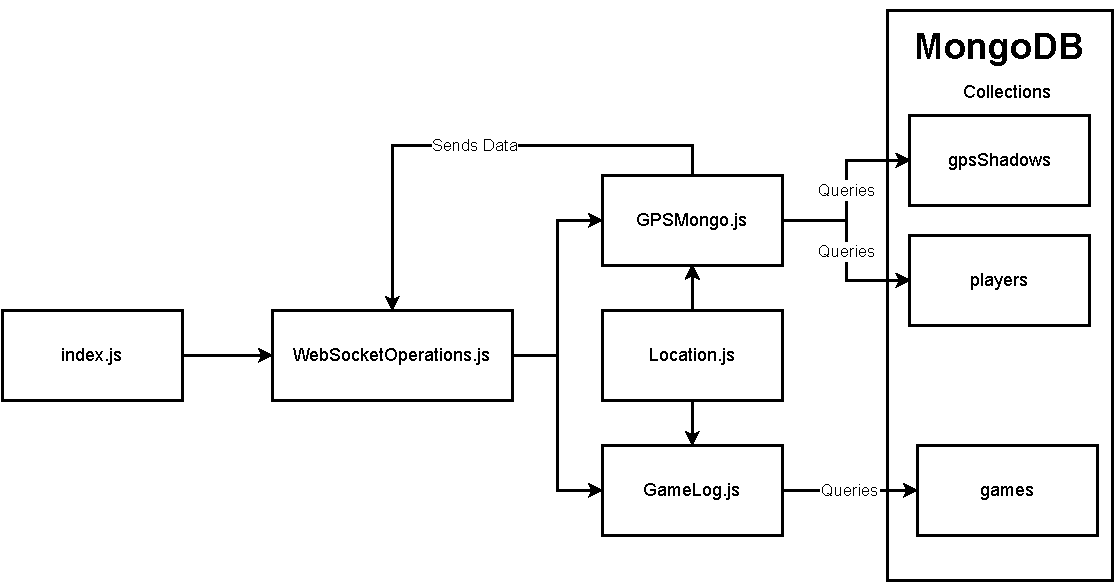
\includegraphics[width=\linewidth]{images/serverSideOverview.pdf}    

    \caption{
        The diagram shows the main flow of files from the server. All requests start at index.js which are
        then processed by the WebSocketOperations.js file. This file will call methods in either the GPSMongo
        and GameLogMongo.js files which make the queries to the MongoDB database.  
    }

    % use the notation fig:name to cross reference a figure
    \label{fig:serverSideOverview} 
\end{figure}


\subsection{WebSocketOperations.js}
As I mentioned in section \ref{serverOverview}, the WebSocketOperations.js file is the main base of operations for
the rest of the game. Whenever a user connects to a server, the methods inside the WebSocketOperations class will take
the user's details like their phone brand and model and then returns them with an id. This id is attached to the connection
object that I could use to keep track of which player is sending the message. The WebSocketOperations.js file is also
responsible for keeping track of whether a game is running or not. If the user were to press the start game button on the
user interface, then the class will run the various methods to work out who will be the chaser.

While the game is running, the WebSocketOperations class will also do some background tasks to make sure that no
player would have an unfair disadvantage while playing the game. The most important task is to have time sync for
the overall game time and when a player ends their jail time. This works by having a background asynchronous method
that counts out 30 seconds. When that time is up, the server will broadcast the current time to all of the players.
I thought that this was necessary due to the fact that while I had a working timer on the User Interface, I would
notice that the times would get out of sync with the other players. I also wanted to ensure that both the jail time
and the game as a whole would end for both players at the same time to avoid any problems or glitches that could happen
if one player was still in the game and another was outside the game. The server allowed me to address any syncing
problems on the mobile app.

As well as keeping the time of the game, the WebSocketOperations.js file has a lot of other systems in place for enforcing the
rules of the game. One of the main parts of my design for the game was that a Chaser would not be allowed to see the Runner's
location if the game was in Jail Time or whether the player was in a Shadow. I managed to implement this rule by making
a function within this file that executes whenever a phone sends a location object. This was especially useful as I could
use it to ensure that locations would always go to the logging database, but will only go to the chaser player if a certain
condition was met.

\subsection{The MongoDB collections}
\label{mongocollections}
Most of the operations offered in the WebSocketOperations.js file are handled in either the GPSMongo.js or the GameLog.js
files. These contain the classes that actually query the MongoDB databases. The database is hosted on a seperate
server on my Railway.app setup. The main benefit of this is that I can directly access my database using a Python
script. However, to reduce the chances of unauthroized users accessing my server, I ensured that all of the credentials
were stored in environment variables and were not exposed in neither the code nor in any server logging system. The
next paragraph will go over the various "collections" that I created to implement this project.

As I mentioned in section \ref{implementationDatabase}, what would be a table in SQL based databases are known as collections in MongoDB.
In my project, I made use of three main collections. These were "players", "gpsShadows" and "games". When a game is being played, the most
important collection is the "players" collection. When a player is connected, a query is sent to this collection which gives back a player id.
We then add the id to the sender's "client" object. This means we can query the right player in the database, I also store the players state,
current location and phone manufacturer (the last one is mainly for logging purposes). If a player was to disconnect, the server will give
them 30 seconds to reconnect before the data is deleted. I put this failsafe in because I would get errors from my phone app saying
that it disconnected from the WebSocket after 5 minutes.

The players collection was also useful for implementing the catching mechanic (see section \ref{catching} for the design). Originally I had planned to put this on the mobile side
as the chaser was able to see the real time locations of the other players, however I found that constantly querying the distance function
on the LocationManager API was affecting the performance of the game. Thankfully, MongoDB offers geospatial queries which allowed me to
easily get data points within a certain radius. To check whether a runner player was in the catch radius, I used the query shown in
listing \ref{lst:catching} to get a list of players within the radius. I then created an array with the results. If the array length is greater
than 0 then we send a message to the WebSocketOperations.js file to turn the captured user into a Chaser.

\begin{lstlisting}[language=javascript, float, caption={The Geospatial query used to implement the catching mechanic. The \$ne key is the way to make a not equals query.}, label=lst:catching]
    const query = {
            _id: {$ne: chaser._id},
            location: {
                $near: {
                    $geometry: {
                        type: "Point",
                        coordinates: [chaser.longitude, chaser.latitude]
                    },
                    $maxDistance: 5
                },
            }
        }
    console.log(query);
    const playersToCatch = await this.userCollection.find(query).toArray();
\end{lstlisting}

Another collection that I created was the "gpsShadows" collection. While this wasn't as useful a collection in the final product, 
it was very useful for my initial analysis section. As the name suggests, it stores previously recorded GNSS shadows in both previous
games and during my initial analysis as discussed in Chapter 3. The criteria for a location to be put into this collection was for
a error reading to be at 6 meters or higher. During the development of phase 1, I was hoping to use this collection to give the runner
a view of some shadows that were found in previous games using a query like listing \ref{lst:catching}. However, like having the catching
on the mobile phone, there were performance issues which made the game unplayable and would have given a runner player a bad experience.

The final collection that I created was the "games" collection. This collection's purpose is to store the game logs within a game. For example
it stores the time that a user was the runner, how long the user was a chaser or runner, where the players went and the locations of where the
players were caught. I also logged some data like the brand name and model of the phones that people were using. While this data doesn't affect
how the game is played, it gives me a lot of data which can help aid my overall evaluation. Whenever a game is started, a brand new game object
is added. It then creates an array of objects for each player. Each location has the latitude, longitude, accuracy, noise Ratio and the minimum
accuracy over time. A lot of the quantitative data discussed in chaper 6 was sourced from this collection.

In order to gain access to the database, I needed to connect it to my server. To do this I created two main JavaScript classes to handle the
communication between the database and the rest of the server side files. I use the GPSMongo.js file to query the "players" and "gpsShadows"
collection and I used the GameLogMongo.js file to query the games collection. These files contain the main methods which carry out the queries
that the WebSocketOperations.js file needs. I did this to ensure that the WebSocketOperations file wouldn't become too big and to ensure that
it's responsibility was mainly focused on processing the WebSocket Messages, therefore satisfying the Single Responsiblity in SOLID.


%==================================================================================================================================
\chapter{Phase 1 Evaluation}
\label{Evaluation} 

In this chapter I will go over the process and results from my two rounds of evaluations.

\section{Process}
The game was tested during the week commencing 23rd January 2023 involving volunteers with a range of Android phones. I set up multiple two player
games that were played around the main building, the cloisters and the surrounding area. Each game lasted 15 minutes where I collected the locations
of the players, their GPS Error and the locations where the players were caught. I also noted down the brand and the model of the phone to analyse
how the game worked with different phones. After playing the game, I would ask my participants to fill in a survey with questions including how
fun the game was to play, whether the connection was stable and what improvements could be made in future iterations. I plan to do two phases
with the second phase set to be done in the week commencing the 6th February 2023.

\section{Results}
\label{phase1}

\subsection{Overview}
For Phase 1 I managed to test the game with 8 participants with a total of 6 games played. Games were either played between me and the participant
or between the two participants. Most of the games went well with the exception of two games where the ranges in errors were higher than my threshold
(I will go into more detail in subsection \ref{phase1errorrange}). I was glad to see that there were no problems with overall connectivity throughout
the duration of the game and that the play tests had an overall positive reception.

\subsection{Strategies}
An interesting thing that came out of this evaluation is the different strategies that some participants made while playing the game. At the beginning
of every game I explained to the participants where some of the best locations to find a GPS shadow would be. With this knowledge most participants
went under the cloisters however one person had a better strategy. They managed to find a route through the University Chapel to the opposite
quadrangle without being detected.

\subsection{Error Ranges}
\label{phase1errorrange}
One of the things that I wanted to see was whether the GNSS accuracies on different phones would be consistent or whether it would vary more.
When I was doing my initial walks finding GNSS Shadows, I only used my personal phone (A Samsung Galaxy S21 FE) to get readings. Figure \ref{fig:galaxys21}
shows the ranges in the Error ratings. From the graph I can see that when this phone is in a relatively open area, the error rate remains constant at around 3.8 meters. There
are only a few peaks throughout the duration of the game. Through experience this only happens when I go into buildings or under bridges and in other areas where GPS performance
is expected to decrease. When developing the game I thought that an error of 6 meters or more would have been the threshold for whether a player was in a GPS Shadow or not as I
assumed that it would be constant for every phone.

When running my game on different phone, I noticed that my assumption that the same range of GPS accuracies were true for all phone was incorrect. Figure \ref{fig:oppo}
shows the Error ranges on an Oppo F19. As you can see from the graph, the range of GPS errors were significantly higher and less consistent than the Samsung phone. I also
noticed that the error would rarely go under the 6 meter threshold. This meant that when this phone was the runner, the chaser was not able to catch or see their location
this led to a major balancing issue. This problem was also found with the Samsung Note 9 (Figure \ref{fig:note9}), with this phone I noticed that the error rate would get
as low as 0 but would rarely be within the 3.8 and 6 range. This would result in their marker making big jumps before becoming invisible again.

From these results I can see that the wide range of android phones would lead to a wide range of GPS sensors. This could be due to many factors, from the amount of satellites
visible to simply the cost of the GNSS sensors. I feel that my original assumption would have been better if I had created the app using iOS, since I would only be developing
for a single phone type. The main conclusion that I decided to make is that I need to find a new way of calculating whether a player is in a shadow or not.
The best way to do this is to consider the median value or the lowest value and then adjust my ranges based on that value.  

\subsection{The Catching Mechanic}
\label{phase1catching}
Another major thing that I wanted to was see whether the catching mechanic (Please see section \ref{catching} for more details on how this works)
was working as intended. I feel that this part of the evaluation had some mixed results. The problems mentioned in section
\ref{phase1errorrange} caused problems to this part of the game as well. Mainly because I had implemented it so that if the
runner was in a GPS Shadow, the catcher could not catch the player. Another thing that I noticed was that when two players
were immediately next to each other, their GPS coordinates would be outside the 5 meter radius. This meant that with a lot of
games there were a few lost seconds while the participants tried to move themselves in order to see if they could catch each other.
My theory as to why this happened would have been due to the mutltipath error. This issue came up the most around the Quadrangles
of the main building. Meanwhile the catching system worked better around the Flagpole.

The problems that I found in regards to the catching mechanic tell me that I need to make two improvements in this area. For one
thing, the catching radius needs to be increased. The 5 meter radius was too small for a catch to be registered in most cases. Therefore
I will look into expanding the radius to 30 meters to account for any multipath problems. The second improvement that I will
make is that I will remove the requirement for the runner to be in a high accuracy area, this is because once when I was a chaser,
I found the runner in a shadow area and I couldn't catch them until we moved into a more open area.




\subsection{Survey Results}
\label{phase1survey}
The main aim for the survey at the end of the evaluation was to get a more opinionated view of how the participants
thought the game went and what improvements they would make. I started by giving them a set of statements and asked
them if they agreed or disagreed with the statements. Table \ref{tab:agree} shows the breakdown of the participents'
responses.

Table \ref{tab:agree} suggests that the overall reaction to the game was positive. For example all 8 participants started
that they enjoyed the game with 3 out of 8 people saying that they really enjoyed it. The survey suggested that the experience
playing the game helped them get a better understanding about how the accuracy of their GPS coordinates can change due to different
factors such as hiding in buildings and under bridges. This had an even stronger response with three quarters of the participants
stating that they strongly agreed that the game educated them on GPS accuracy. However, the last two questions which were
about the game connection and the user interface had a more mixed response. The User Interface had 4 people who had a Neutral
opinion. This was mainly due to the fact that each player had a marker which was the same colour. The connection question
was the only question which had people who said that they disagreed with the statement. This was mainly due to the problems discussed
in sections \ref{phase1errorrange} and \ref{phase1catching}. In future iterations I will have another look at the user interface
and I will look into having multicoloured markers.

At the tail end of the survey I gave each participant a list of potential features that I was thinking of implementing in phase 2.
I asked the participants to rank the following proposed features:

\begin{enumerate}
    \item Limits for how long someone stays in a GPS Shadow
    \item A powerup system which are earned when the player stays in high GPS accuracy areas
    \item The Runner being able to see the Chaser all the time
    \item Having a new winning condition. Something along the lines of a last man standing system
\end{enumerate}

From the responses that I recevied, the most popular feature was to have a limitation on how long someone can stay in a shadow with
5 out of 8 of my participants ranking it first. Surprisingly the least popular feature was letting the Runner see the Chaser all the time.
My guess is that the design for the runner type makes the game more tense if you don't know exactly where the chaser is going to be.
I discussed with the players about the limits on how long someone can stay in a shadow and most people said that it was better to have
a more punishing mechanic than a rewarding one in the form of a powerup system to ensure that the runners don't just stay in the same place.

In the final part of the survey I asked the participants whether they had any further comments or feature ideas. One of the most common
feature ideas brought up in this section was to have a different colour of marker to show who is the chaser and who is the runner. Up to this
point I had just used the generic marker in the Google Maps Jetpack API. Another interesting thing that came up was that I should consider
adding a manual catching mechanic as a potential solution to the problems raised in section \ref{phase1catching}. I feel that this could be
a good solution but increasing the catch radius would still be an easier solution and would help teach the participants how GPS errors could
come about.

\begin{table}[]
    \centering
    \resizebox{\textwidth}{!}{\begin{tabular}{|l|l|l|l|l|l|}
    \rowcolor[HTML]{9B9B9B} 
    \textbf{Question}                                                                  & \textbf{Strongly Agree} & \textbf{Somewhat Agree} & \textbf{Neutral} & \textbf{Somewhat Disagree} & \textbf{Strongly Disagree} \\ \hline
    The Gameplay was an enjoyable experience                                           & 3                       & 5                       & 0                & 0                          & 0                          \\ \hline
    The game gave me a better sense of awareness as \\to where GPS accuracy can decrease & 6                       & 2                       & 0                & 0                          & 0                         \\ \hline
    The User Interface Displayed information clearly                                   & 2                       & 2                       & 4                & 0                          & 0                          \\ \hline
    The game connection was stable                                                     & 4                       & 2                       & 0                & 2                          & 0                          \\ \hline
    \end{tabular}}
    \caption{At the start of the survey I gave my participants 4 statements and asked them whether they agreed or disagreed with it. This table shows the results of that survey}
    \label{tab:agree}
\end{table}

\chapter{Phase 2 Design and Implementation}
\label{phase2design}

\begin{figure}
    \label{fig:phase2_ui}
    \centering
    \begin{subfigure}[b]{0.3\textwidth}
        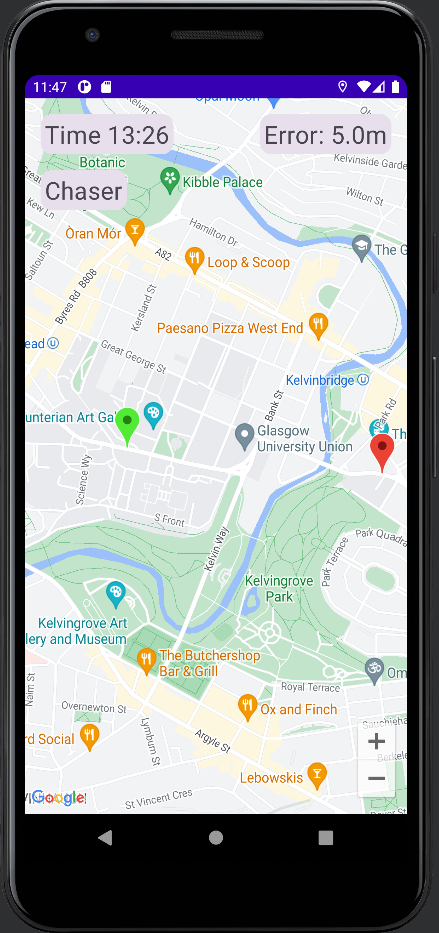
\includegraphics[width=\textwidth]{images/phase2_ui_chaser.png}
        \caption{The Chaser view.}
        \label{fig:phase2_ui_chaser}
    \end{subfigure}
    ~ %add desired spacing between images, e. g. ~, \quad, \qquad, \hfill etc. 
      %(or a blank line to force the subfigure onto a new line)
    \begin{subfigure}[b]{0.3\textwidth}
        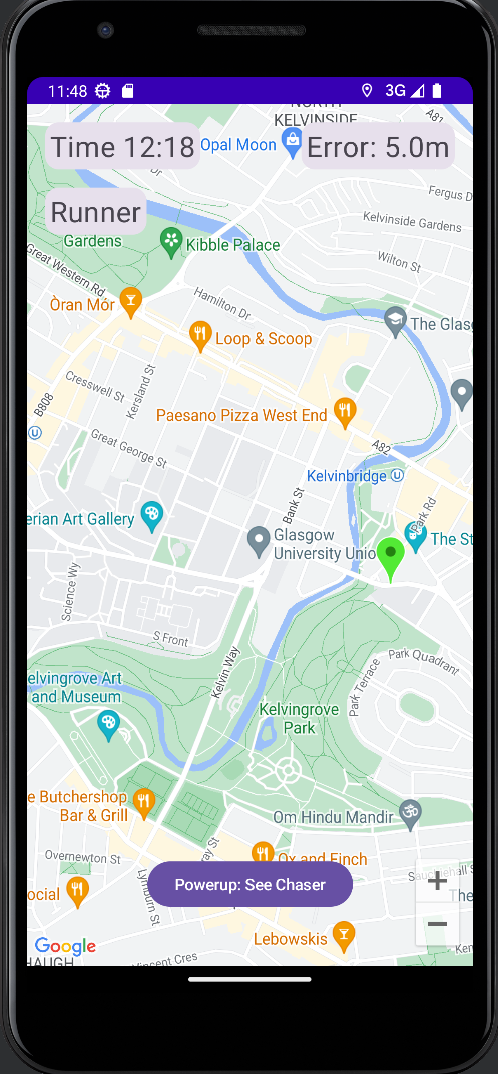
\includegraphics[width=\textwidth]{images/phase2_ui_runner.png}
        \caption{The Runner View}
        \label{fig:phase2_ui_runner}
    \end{subfigure}
    
    \caption{These two screenshots show the User Interface as it was at the end of phase 2. The main
    differences being the new marker for the current player's location.
    }
\end{figure}

\section{Introduction}
In response to the evaluations discussed in section \ref{phase1}, I knew that I needed to make some changes to my app
to improve the game based on the user's feedback. As a lot of the issues raised in the phase 1 evaluation showed that
there were problems that affected the player's enjoyment of the game, I felt that it was important to take a seamless
approach. Some of the seams that I found in phase 1 caused more frustration in my players and they didn't lead to more
interesting ways of interacting with the game.This chapter goes over the four changes that I made during this
iteration of development.

\section{New Player Markers}
The smallest change this phase was in response to feedback raised in the survey of the first evaluation. This was mainly
due to the fact that in the first phase of development, I used the default marker icon from the Google Maps SDK. This
made the game rather confusing for the players. Therefore I decided that I would change the colour of the player marker
to green and I left the marker colour to red for any other players. 

\section{Catching}

\subsection{Design}
\label{phase2catchingdesign}
During my Phase 1 evaluation I noticed that the design mentined in section \ref{catching} was not as suitable due to 
multipath errors(see section \ref{phase1catching} for more details). The main problem being that if the catcher tried
to catch a player, they would have to move around before it would register. For phase 2 I will make a more dynamic design
where the catch radius will increase or decrease depending on how likely a multipath error was able to occur. Uber found
a way to improve their GPS accuracy by making use of the signal noise ratio of each satellite and comparing it to a 3D map.
They found that a high ratio would mean that the sensor is in direct view of a satellite while a low satellite would mean that
the signals were more likely to be obstructed by buildings, trees and other obstables \citep{uberGPS}. While using a 3D map
to improve the catching mechanic is out of the scope for the project, I will take the idea of getting the average SNR. I will
now dynamically increase and decrease the catch radius by dividing 5 from the average ratio (as a number between 0 and 1). My hope
is that if two players are closer together, a catch will be more likely to be registered.

\subsection{Implementation}
For this I implemented the phase 2 design that I had discussed in section \ref{phase2catching}. To implement this design
I decided to create a new class in the GPS package called GPSCatchRadius. Using the LocationManager API in the standard
android library, I was able to get an array of the visible satellites. From then it was trivial
get the noise ratio by using the getCn0DbHz method provided by the LocationManger API \citep{locationManager}. With all
the noise ratios, I took the mean and then normalized it so that it was on a scale between 0 and 1. Once that was done,
I divided 5 by the mean ratio. Then through the LocationWebSocket class, I was able to send the noise ratio.

On the server side, not much needed to change in order to get this feature to work. The only main thing that I needed to
do was change the MongoDB query in listing \ref{lst:catching} to have the maxDistance as the adjusted catch radius. The
only other thing that needed to be done was to update the Logging database to collect the noise ratio. This was mainly
so that I could analyse any trends in the noise ratio data in order to inform me of other features and improvements
in future phases.

\section{Shadow Threshold}

\subsection{Design}
As mentioned in section \ref{phase1errorrange}, I noticed that there were differences in the GPS error rates
in various versions of android phones. This meant that some players were invisible for long periods of the game.
In order to solve this problem, I decided that there needed to be a dynamic approach to calculating whether a
phone is in a shadow or not. The two ideas that I considered was either to take the mean error and multiply that by 2
or to take the minimum error and multiply it by 2. In the end I decided to go for the latter as I remembered when 
I was walking around finding GPS error rates, I found that the mean error rating would have skewed towards larger
error rates. While there can be problems with having the minimum error rate, I felt that it was the best baseline
as you would expect that the minimum GPS error rates to be in more open areas. I also felt that it followed if the
recorded error rates were twice the baseline then that would be a significant enough range to safely say that
the sensor is in a Shadow.

On the chaser side, I noticed that because I had also linked the ability to catch a runner to their error rate, it
meant that the runner would be able to evade capture by just staying in shadow areas. There were some occasions
were the participants physically caught the runner, but it wasn't registering on their phone as they were above the
error threshold. Therefore I decided that the shadow threshold would no longer affect whether a chaser can catch the
runner or not. I feel that this will make the game more fair and would be a way of rewarding the chaser for not
relying entirely on the map when locating the runner.

\subsection{Implementation}
Implementing this design was trivial with only a few further considerations. One of the main one was that I
needed to ensure that the minimum error rate calculation was done every time that a new location was recorded.
I had to do this in case the player was starting the game in a shadow rather than in open terrain. Another
small consideration that I implemented was a check to ensure that the minimum error radius could not be zero.
This was because the person with a Samsung Note 9 stated that their phone had briefley reported an error of 0 
and figure \ref{fig:note9} also shows such an abnormal error rate. Therefore I decided to add that failsafe to
ensure that a player could not be invisible all the time.  

\section{Powerup System}

\subsection{Design}
While I felt it was important to fix some problems that were raised in the first evaluation, I also
wanted to implement one of the proposed features at the end of the survey. Upon looking at the feedback
I decided that I wanted to implement a basic powerup system. For this phase I designed one power up for
the runner, this was to simply be able to see the chaser's location for a few seconds. I feel that although
the old design gave a lot of suspense to the game, I was interested to see how the player's strategies
would change with this new feature. Since some people in phase 1 would mainly focus on staying in shadowy
areas, I decided to make this powerup unlock after a full minute of being in more open areas. I felt that
this would add a level of risk to the game as the runners would have to go out in the open to get further
information on where the chaser was.

\subsection{Implementation}
In order to implement this feature, I started by creating a button element at the bottom of the runner view.
I did this by creating a simple button element with the words "See Chaser" with a progress bar at the bottom.
The progress bar would increase whenever the runner updated their location and they were below their shadow
threshold. When the runner has had 30 location updates in high signal areas, the button will become clickable.
When the user clicks on the button, they will be able to see the Chaser's location on the map for 3 seconds before
the powerup button resets the progress bar.

On the server side I decided that this powerup would be implemented by a simple HTTP request rather than through
the WebSocket system for all other client communications. My main reasoning for this was that since the client
updates their location every 2 seconds and the powerup would only show the chaser for 3, there wouldn't have been
a point in setting up another action in the WebSocketActions class. Therefore I just created the "/chaserLocation"
endpoint where I simply get the location from the database and send the latitude and longitude in a JSON object.

\chapter{Phase 2 Evaluation}

\section{Overview}
Two weeks after the first phase of evaluations, I made improvements to the overall design (See chapter \ref{phase2design} for an overview
of what has changed). The format of the evaluation was similar to the first, with the same participants. For this evaluation I especially
wanted to test if my improvements had fixed the problems raised in the first phase. These being the ranges in accuracy between different
phones and the catching mechanic being affected by multipath errors. Another feature that I was testing out was the brand new powerup
system that I created. The next few subsections will examine whether the improvements succeeded or not.

\section{Error Ranges}
This time, the game worked on a dynamic basis rather than the static version of before. Instead of the shadow threshold being
6 meters, it would now be twice the current recorded minimum accuracy. For example if the minimum score was 3.8, it would now
only be in a shadow if the GPS area was 7.6 meters in error. My hope was that this would end the inbalance in the game were
phones with a higher average accuracy would get an unfair advantage over other players.

To see if this was a success, I looked at the amount of time that a player would be in a shadow vs when they were out in the
open. The assumption was made that the player was a runner throughout the duration of the game, this was because I did not have
information on whether the player was a chaser or not in the logging system. I used the data based on the three phones that I 
analysed in the last evaluation of the error ranges (See section \ref{phase1errorrange} for more detail). This was because I wanted
to see how it worked on an accurate phone (Samsung Galaxy S21 FE) and the phones where I noticed the most variance in error range (The Samsung Note 9 and the Oppo F19).
My hypothesis was that there would be a reduction in the amount of time in shadow for each type of phone. This means that there would be
more times where a player would be more visible during the game and would only be invisible when they are in a shadow area.

Figures \ref{fig:shadownote9}, \ref{fig:shadowoppo} and \ref{fig:shadows21} show the shadow results for the Samsung Note 9,
the Oppo F19 and the Samsung Galaxy F21 respectively. I feel that the results are quite mixed, where I would say that the
Samsung Note 9 (\ref{fig:shadownote9}) is the only one that had an improvement overall where there was an increase from
44.8\% in phase 1 to 60\% in phase 2. This means that overall the player is not considered to be in shadow for the majority
of the game. However the Oppo F19 (\ref{fig:shadowoppo}) told a different story. I actually saw that the amount
of time in "high GPS" areas decreased overall from 59.6\% to 31.7\% in phase 2. This means that they would have been more
invisible than in Phase 1 meaning that they would have an even greater advantage. The same problem but in reverse happened
to the Samsung Galaxy S21 FE where the in open time increased to 100\%. Esentially meaning that the player would be visible
for the whole game.

These mixed results suggest to me that either the problem of someone being invisible was not as great as I perceived it in
the phase 1 results suggested. Another thing that it has suggested to me is that this approach also has some flaws. While
it has somewhat improved the error ranges there are times where it has been worse. This leads me to the conclusion that it might
have been better to constantly check the mean or take the standard deviation rather than just a flat rate for all error ranges.
If I have more time to implement a new system, I would look into making a new variance based system.

\section{Catching Feature}
\label{phase2catcheval}
Another major improvement that I implemented was a new catching system where the catch radius can increase or decrease based
on the satellite noise ratio based on the method described by \cite{uberGPS}. For this evaluation I was hoping that the catching mechanic would be more helpful to play when
accounting for multipath errors.

In order to put this feature to the test, I took some Qualitative and Quantitative methods into account. Firstly I made sure to log both
the noise ratio and the size of the catch radius over the course of each game. To see whether this behaviour is the same over every phone
I made a seperate graph for each of the three phone types that I have used in both phase 1 and 2 to see how the noise ratio is affected
with different phone. During the game I will observe what happens when a participant catches another player. I will use this to see if
this new approach works in practice.

Figures \ref{fig:opponoiseandcatch}, \ref{fig:note9noiseandcatch} and \ref{fig:s21noiseandcatch} show a side by side comparision of the
noise ratio compared with the catch radius for the Oppo F19, Samsung Note 9 and the Samsung Galaxy S21 respectively. Like the Error rates in
phase 1 (see \ref{phase1errorrange}), the ranges of noise ratio vary based on the kind of phone, leading to the same observation happening in
the size of the catch radius. For example the Oppo F19 seen in figure \ref{fig:opponoiseandcatch} shows that there is a big range between a ratio
of roughly 0.35 and under 0.1. Around 100 seconds in to the game, the phone experienced a massive decrease in the ratio, leading to the catch radius
to be larger than 60 meters. This gave the player a larger radius in order to catch players. During this game, one player who was using the Samsung
Galaxy Note 9 was caught in the cloisters while the person playing with the Oppo was in the Gift Shop. This lead to some rather interesting ideas
of how stealthy other players can be in order to gain an upper hand in the game.

The Samsung phones seemed to be more consistent in their noise ratio and catch ratio. For example the Samsung Note 9 (\ref{fig:note9noiseandcatch})
shows that the highest catch radius was 16 meters while the Samsung Galaxy S21 (\ref{fig:s21noiseandcatch}) had a maximum of 15 meters. Both phones
also recorded the smallest catch radius of around 9 meters. The fact that these results were so close was surprising considering that the Note 9
had a significantly low range of accuracy compared to the Samsung Galaxy S21. While there is a chance that the person with the Oppo F19 had a different
strategy, it could also be due to the difference of GNSS sensor that is causing the problems. The main reason I think this is that the highest
value of signal noise ratio in the Oppo F19 was around 0.35 wheras with the Samsung phones 0.35 wass the lowest value. Therefore as with the accuracies
in phase 1, there is a variance between the different phones.

While these ranges may be seen as a problem if a seamless approach was made when designing the game, it can also be seen as a benefit. For
example, a mechanic could be that phones with a higher chance of having low noise ratios could be seen as more threatening since their catch
radius could become large if they are in the right positions. This could add new stakes to the game where people with better and more accurate
GNSS sensors have to be quick and aim to get as close to the player as possible while a runner would have to ensure that they get as far away
as possible from a chaser with a phone with a larger catch radius.
\begin{table}[]
    \centering
    \resizebox{\textwidth}{!}{\begin{tabular}{|l|l|l|l|l|l|}
    \rowcolor[HTML]{9B9B9B} 
    \textbf{Question}                                                                  & \textbf{Strongly Agree} & \textbf{Somewhat Agree} & \textbf{Neutral} & \textbf{Somewhat Disagree} & \textbf{Strongly Disagree} \\ \hline
    The Gameplay was an enjoyable experience                                           & 2                       & 2                       & 0                & 0                          & 0                          \\ \hline
    The game gave me a better sense of awareness as \\to where GPS accuracy can decrease & 3                       & 1                       & 0                & 0                          & 0                         \\ \hline
    The User Interface Displayed information clearly                                   & 2                       & 2                       & 0                & 0                          & 0                          \\ \hline
    The game connection was stable                                                     & 0                       & 4                       & 0                & 0                          & 0                          \\ \hline
    I could catch my opponent by simply walking up to them                                                    & 1                       & 3                       & 0                & 0                          & 0                          \\ \hline
    The 'See Chaser' powerup helped me form a different strategy                                                     & 3                       & 0                       & 1                & 0                          & 0                          \\ \hline
    \end{tabular}}
    \caption{Like phase 1, I gave my participants a brief survey at the end of my evaluation. I gave the users some of the same questions as before along with two other questions
    to guage how useful they thought the new features were.
    }
    \label{tab:agreephase2}
\end{table}

\section{Survey Results and the Powerup System}
Just like at the end of my Phase 1 evaluation, I wanted to gauge how interesting and informative the game was.
This time round I had a lower cohort of people with only 4 people responding. I mostly evaluated my game with
the same people as the first phase of evaluations. Overall, most people said that the new features improved the
game. This section will go over the quantitative and qualitative data that I found when carrying out my survey.

I started my survey by asking the participants to rate their opinions on the same 4 statements as in the previous
evaluation. Table \ref{tab:agreephase2} shows the results of this survey. Of the people that responded, all of the participants stated that they agreed that the game was an
enjoyable experience, with there being a more 50/50 split when compared to the previous phase. The same ratio
of people said that they strongly or somewhat agreed with the idea that the game taught them more about the accuracy
of GPS. 3 out of 4 stated that they strongly agreed with the statement. One of the best improved statements was
'The User Inferface Displayed information clearly' where all participants said that they agreed with the statement.
This was especially good since in the last evaluation, 50 percent of participants gave a neutral response. Finally
I got a full 100\% of participants stating that they somewhat agreed with the fact that their connection was stable
throughout the course of the game.

After that, I gave the participants two new statements which focused on the Catching Mechanic and the new powerup
system. Looking at the last two statements of table \ref{tab:agreephase2}, I found that 3 out of 4 of the
participants said that they somewhat agreed with the fact that the catching mechanic had improved with one
person stating that they strongly agreed with the statement. The final question I asked was whether or not
they agreed that the "see chaser" button improved the game. The responses were positived with 3 out of 4
saying they strongly agreed with only one person saying that they had no real opinion on the statement.

At the end of the survey I asked my participants some Qualitative questions to get some more details about
their experience. Like the first phase, I asked whether there were any balancing issues when playing the game.
Out of the quotes recorded in section \ref{phase2balance}, the main issues were to do with the catch radius,
for example one person said that the catch radius was "too big" and another said that "the chaser was able to catch
me from far away". This ties into the issues that I reported in section \ref{phase2catcheval} where the catch
radiuses would become really big over time. While the participants say that it might affect the balance of the
game, I still feel that there could be potential for a fun game mechanic where different phones will be able
to take out runners at larger distances than other phones.

Finally, I asked my participants to give any other feedback that they may have about the overall gameplay
and the things that I could do to improve. Some things that came up in this question (full results on 
section \ref{phase2generalfeedback}) were that the users wanted to see their catch radius on the map.
Other comments stated that the powerup feature was really useful with one participant saying that
they "found the powerup useful as a runner". Other participants told me that the powerup feature
was really useful in informing their decisions. Over the course of the games I observed that people
had altered their strategy because of this feature. Chapter 




%==================================================================================================================================
\chapter{Conclusion}
\section{Summary}
Throughout the course of this project and this dissertation, we have explored the concept of seamful design.
This is where we take the limitations of a system and exploit them to make them a core feature. In this
case we have gone over the limitations of both GPS and other GNSS systems. In chapter \ref{background},
we gained an understanding of some of the factors that affect the accuracy and error rate. Once we knew the theory
behind how GPS works, we did some experiments where we tested these concepts by going to multiple environments to
see the differences in accuracy. We used this experiment to determine whether to use pure satellite systems
or the usual GPS and WiFi locations found on most smartphones. Through this experiment, I found that using
pure satellite navigation would make for a more interesting game as it was more consistent as to where shadows
could be found. I also concluded that the game would have to be played in a more urban area where signals from
satellites were more likely to be obstructed.

Once I had done my analysis on where GPS signals can decrease, I started an iterative design and development
aproach to creating a game. During phase 1 I started by brainstorming ideas for a game and then progressively
buidling on ideas that were feasible and would work within the time frame required. I decided on creating a
tag game where a "chaser" would have a real time location of a "runner" unless they were in areas with a high
error rate. In chapter \ref{phase1implementation}, I went over the technologies that I used to implement the
game. I also went over the alterations that I had to make from the design to ensure that the game was an enjoyable
experience. In chapter \ref{Evaluation} I tested out my implementation by getting multiple participants to play
a game around the University campus. While the game was received well, I noticed that the assumptions in my 
design and implementation were wrong when I noticed that different phones had different ranges in error rates.

For Phase 2, I decided to take a seamless approach. This was mainly due to the lessons learned from the previous
evaluation. For this phase I made several improvements, the most important of these were having a dynamic shadow
threshold based on the minimum error radius and a new catching mechanic based on the satellite noise ratio. I
also did some User Interface improvements like changing the colour of the player marker. Another major improvement
was a powerup system where a runner player will be able to see the chaser after being in an open area for long enough.
I did another set of user evaluations which led to mixed results. For example the improved shadow thresholds made some
phones more invisible than before, to having some phones being visible during the entire course of the game. I however
found that the users thought that the new iteration was an overall improvement to the previous version.

\section{Future Work}
Due to the limited time that I had to complete the project, there were still some things that I would want to do
to ensure that the game was a better experience. Over the next few paragraphs I will go over some of the ideas
that I have to improve the game if I were to carry out a phase 3 for the project.

Throughout my development, I mainly considered the core mechanics of the game rather than how the players would win.
Initially I had put in my design that the winning condition was that the person who was a runner for the longest time
would win. I however, hadn't managed to get my implementation to work fully. While I have the logging capabilities to
decide who won, I have no way of telling the winner if they won or not. If I were to have further time, I would have a
further look into what conditions a player would need to win and also how they would get feedback for how they would win.

From my findings in section \ref{phase2catcheval}, I noticed that the noise ratios differed based on different phones.
This felt a lot like my findings with shadow thresholds in phase 1. However I feel that there are a lot of opportunities
to be seamful with this discovery. For example, I could implement a character based system with specific abilities like the
popular video game \emph{Overwatch} \citep{overwatch}. A feature that could take this idea is that each phone will have
a class based on how big their catch radius can get. This could mean that a player with a larger noise ratio could be more
threatening to a runner than one with a small catch radius. I feel that this could lead to more interesting strategies if
this were to be implemented correctly.

Another lesson that I learned from phase 2 is that while the new shadow threshold did allow weaker phones to
be seen from the chaser, it came at the expense of some of the more stronger phones. While I could integrate
that into a character ability game, I might look into other ways to improve the shadow threshold system. One
idea that I have is to use the median and standard deviation to decide the threshold rather than the minimum
accuracy times 2.


\section{Reflection}


%==================================================================================================================================
%
% 
%==================================================================================================================================
%  APPENDICES  

\begin{appendices}

\chapter{Phase 1 Design Ideas}

\begin{figure}
    \centering
    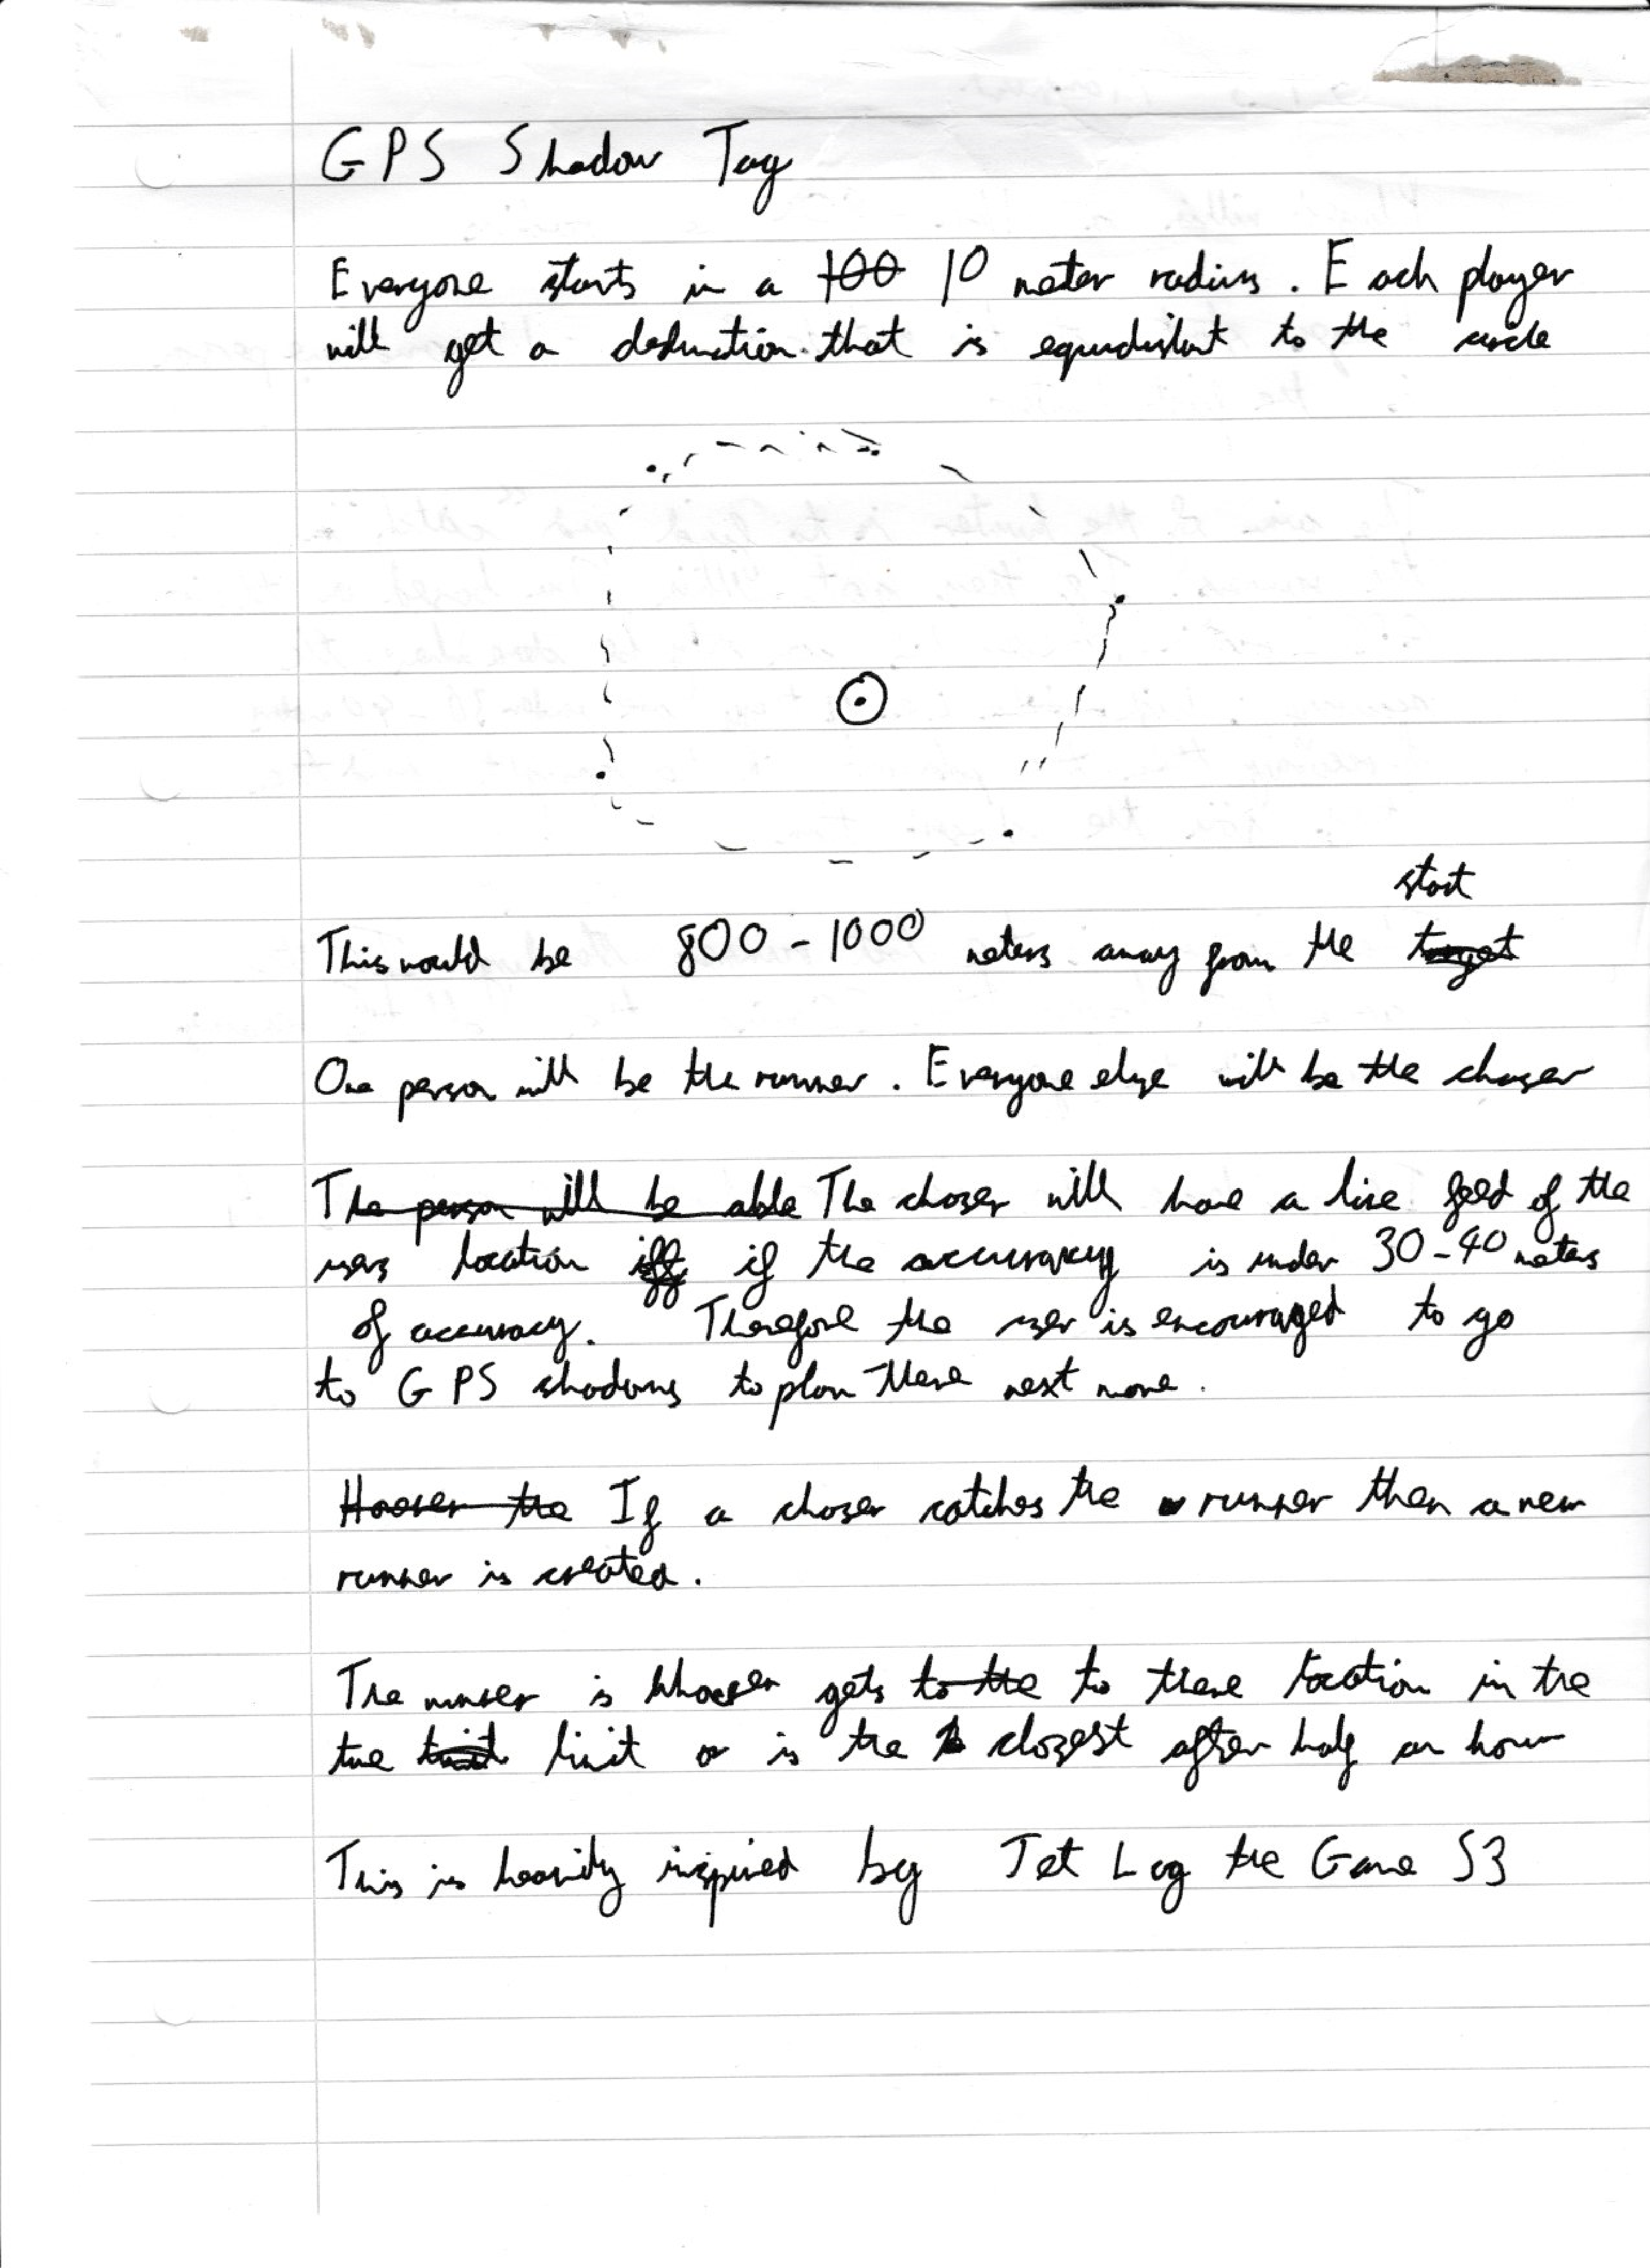
\includegraphics[width=\linewidth]{images/idea1.pdf} 
    \caption{My rough paper draft of idea 1}
    \label{fig:idea1}
\end{figure}
\begin{figure}
    \centering
    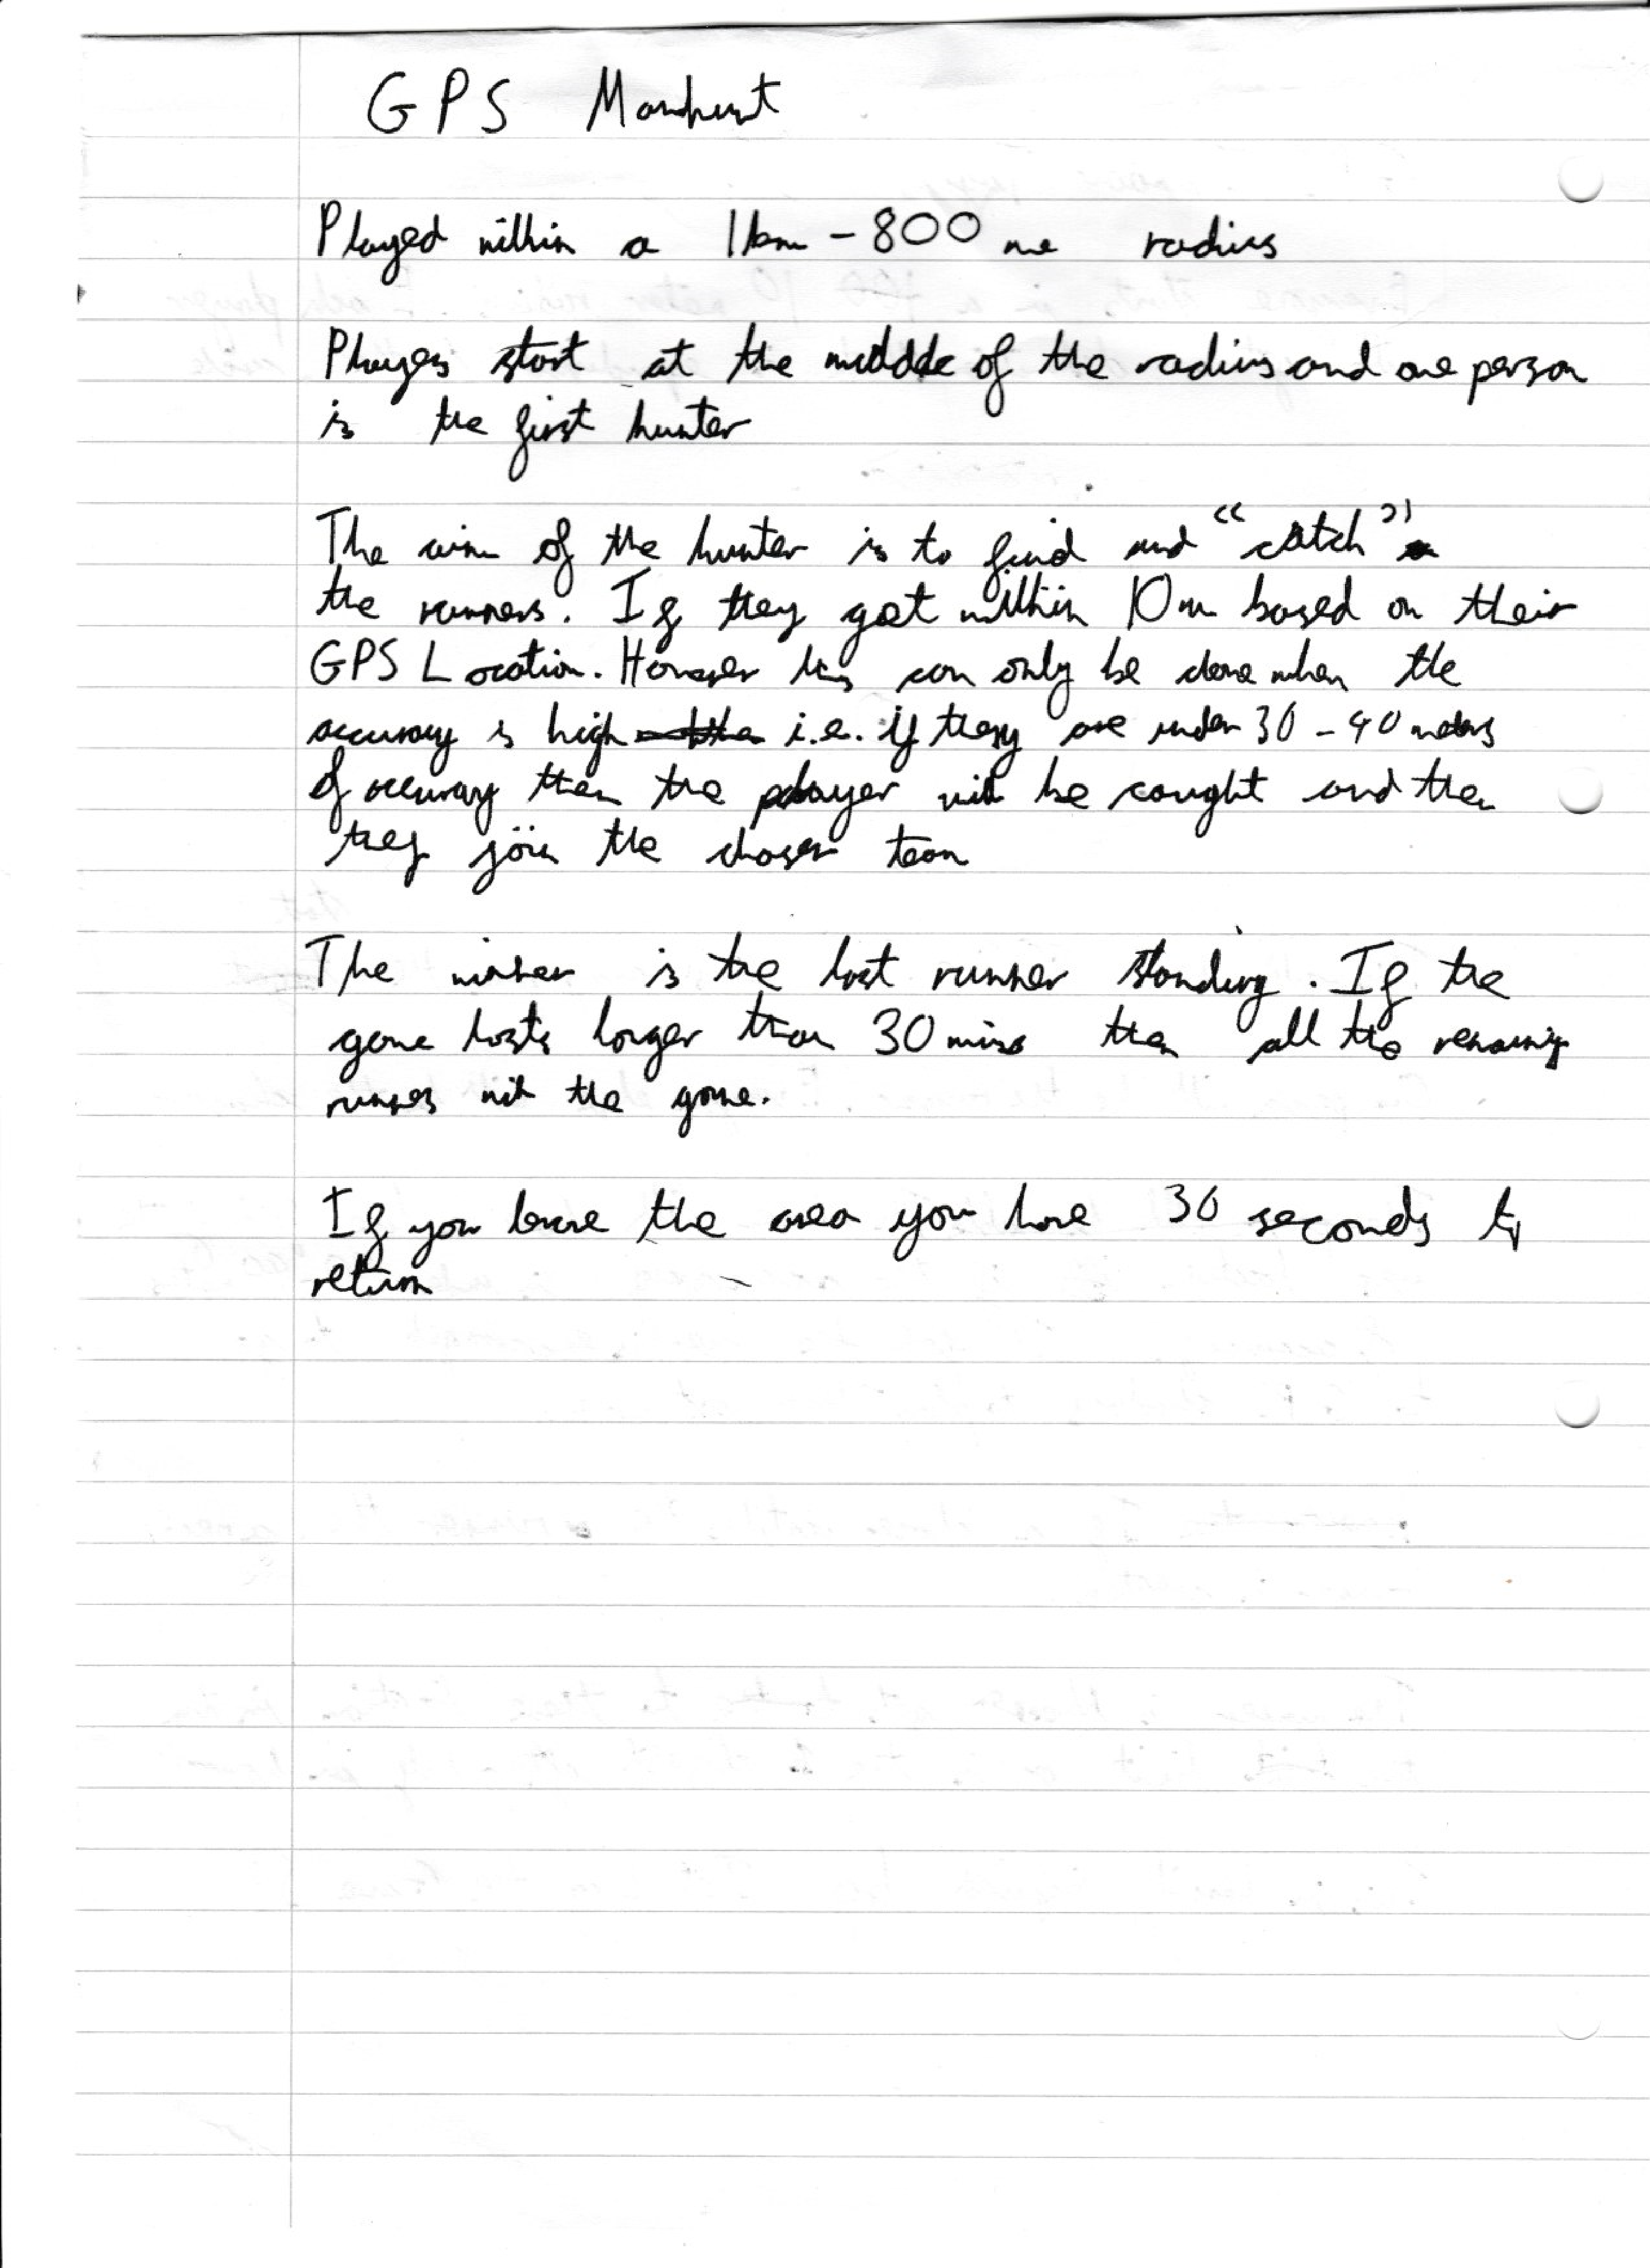
\includegraphics[width=\linewidth]{images/idea2.pdf} 
    \caption{My rough paper draft of idea 2}
    \label{fig:idea2}
\end{figure}

\chapter{Phase 1 Evaluation Graphs}

\begin{figure}
    \centering
    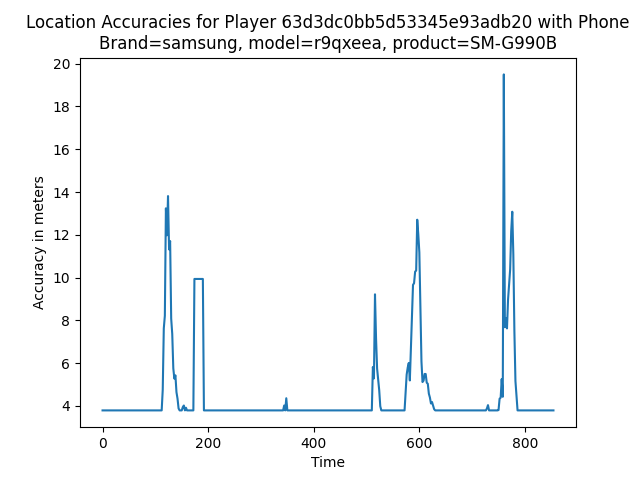
\includegraphics[width=0.8\linewidth]{images/my_phone.png} 
    \caption{The Error ranges found during a game using a Samsung Galaxy S21 FE}
    \label{fig:galaxys21}
\end{figure}
\begin{figure}
    \centering
    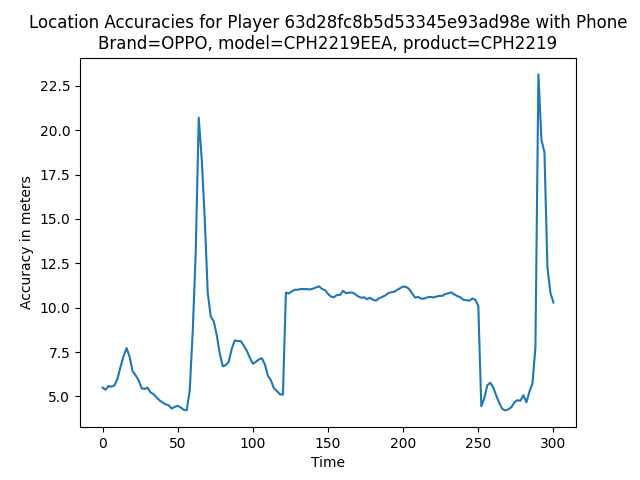
\includegraphics[width=0.8\linewidth]{images/oppo.png}
    \caption{The Error ranges found during a game using an Oppo F19}
    \label{fig:oppo}
\end{figure}
\begin{figure}
    \centering
    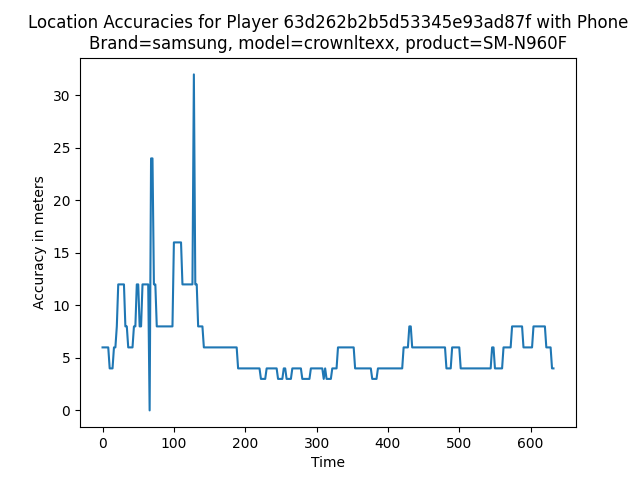
\includegraphics[width=0.8\linewidth]{images/note9.png}
    \caption{The Error ranges found during a game using a Samsung Note 9}
    \label{fig:note9}
\end{figure}

\chapter{Phase 1 Qualitative Data}

\section{Do you feel that there were any balance issues in the game?}

\begin{itemize}
    \item Only balancing issue I think was the duration of the jail time and the difference between the GPS accuracy in the phones.
    \item I felt like runner should also be able to see the chaser. Maybe not always but every 20 seconds.
    \item Too hard for chasers to catch runners due to poor GPS error.
    \item not really
    \item Difference in phone GPS
    \item No
    \item No both players had similar error radii. Felt very balanced.
\end{itemize}

\section{Do you have any other comments, feature ideas or feedback?}

\begin{itemize}
    \item Do you have any other comments, feature ideas or feedback?
    \item Maybe better pointers graphics for runner and chaser.
    \item Differentiate location icons. Custom timer. Manual catching.
    \item Was a really fun game to play! Some features which would be nice to see is: - different markers for chaser and runner - customisable game timer - button to manually say a runner has been caught
    \item Was fun
    \item 	Different colours for the chaser and runner location pins Maybe restrict the play area like a battle royale game Adding directional arrows to players pins
\end{itemize}

\chapter{Phase 2 Evaluation Graphs}
\begin{figure}
    \centering
    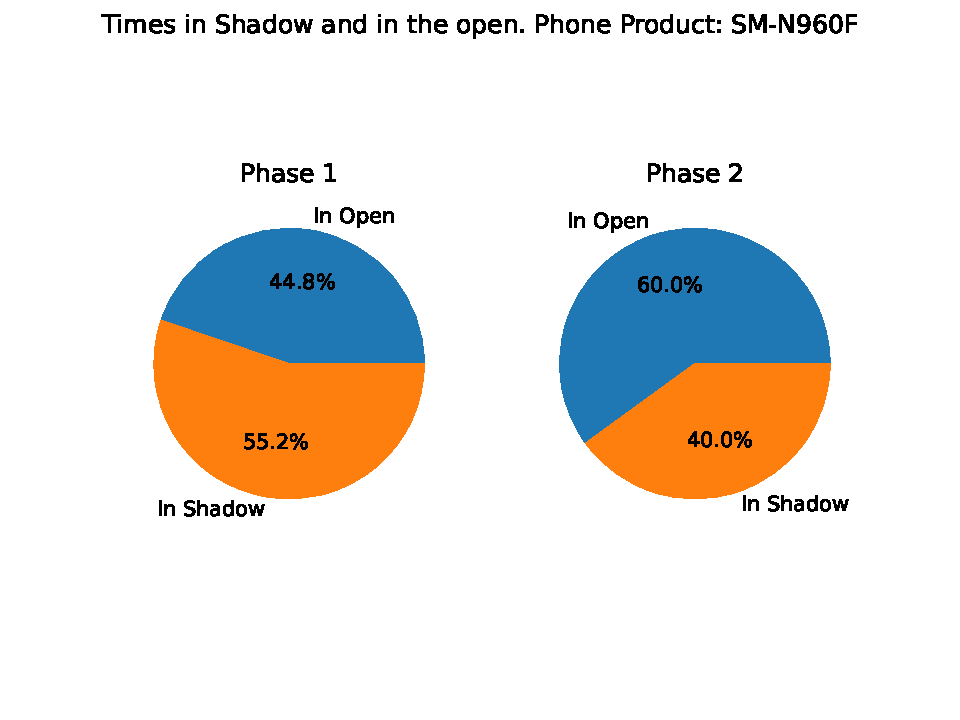
\includegraphics[width=0.8\linewidth]{images/SM-N960F_piechart.pdf}
    \caption{The times in a shadow and in the open during a game using a Samsung Note 9}
    \label{fig:shadownote9}
\end{figure}
\begin{figure}
    \centering
    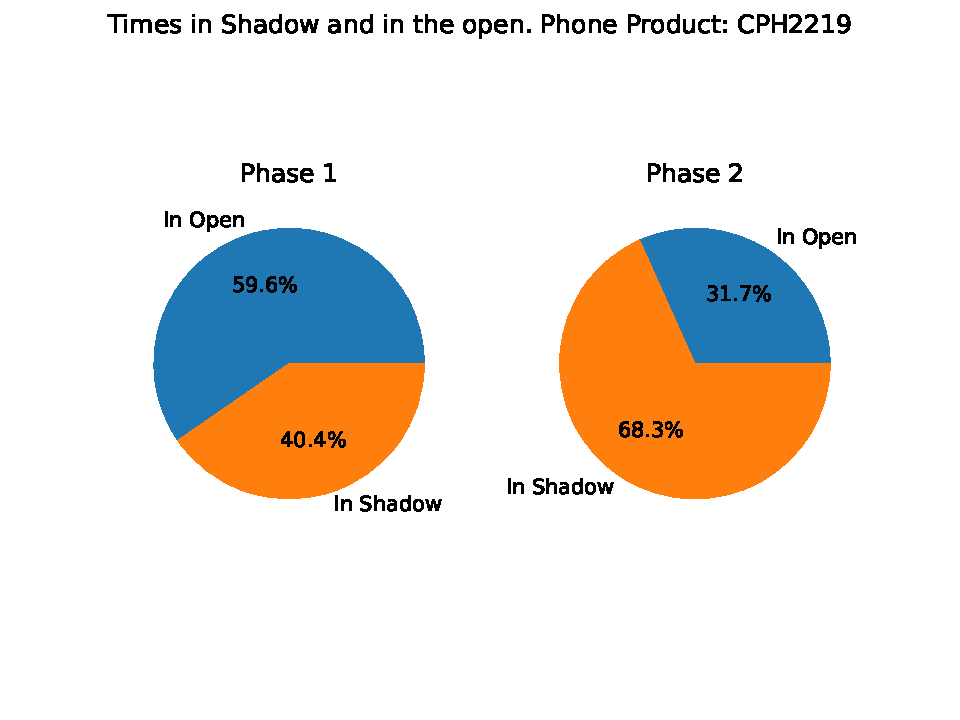
\includegraphics[width=0.8\linewidth]{images/CPH2219_piechart.pdf}
    \caption{The times in a shadow and in the open during a game using an Oppo F19}
    \label{fig:shadowoppo}
\end{figure}
\begin{figure}
    \centering
    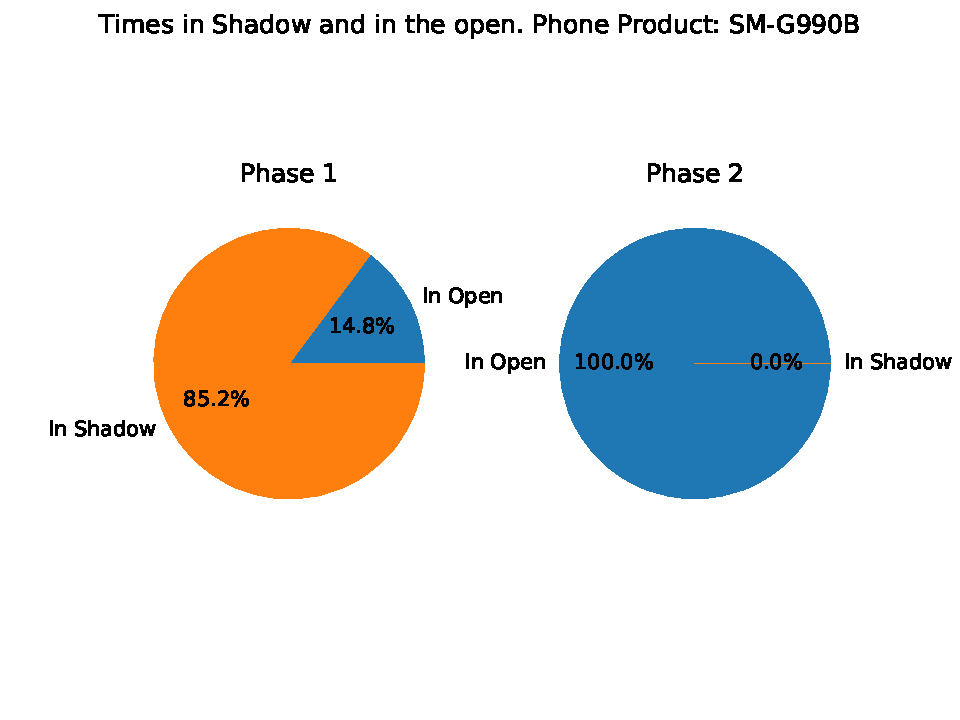
\includegraphics[width=0.8\linewidth]{images/SM-G990B_piechart.pdf}
    \caption{The times in a shadow and in the open during a game using a Samsung Galaxy S21 FE 5G}
    \label{fig:shadows21}
\end{figure}
\begin{figure}
    
    \centering
    \begin{subfigure}[b]{0.48\textwidth}
        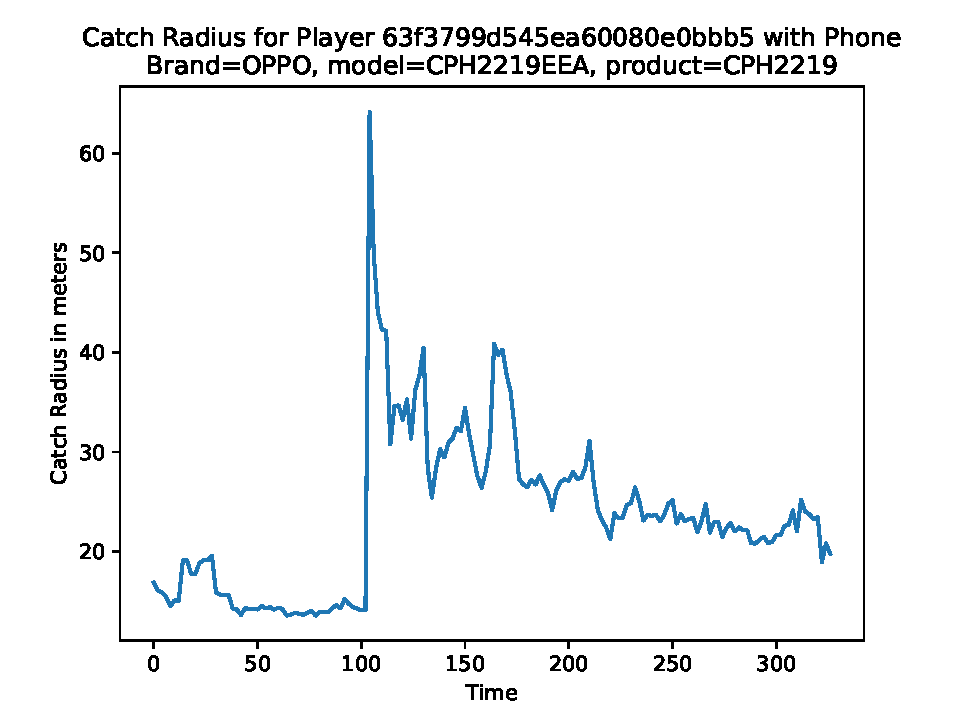
\includegraphics[width=\textwidth]{images/OPPO-CPH2219EEA-122-radius.pdf}
        \caption{The Chase Radius over the duration of the game}
        \label{fig:oppocatchradius}
    \end{subfigure}
    ~ %add desired spacing between images, e. g. ~, \quad, \qquad, \hfill etc. 
      %(or a blank line to force the subfigure onto a new line)
    \begin{subfigure}[b]{0.48\textwidth}
        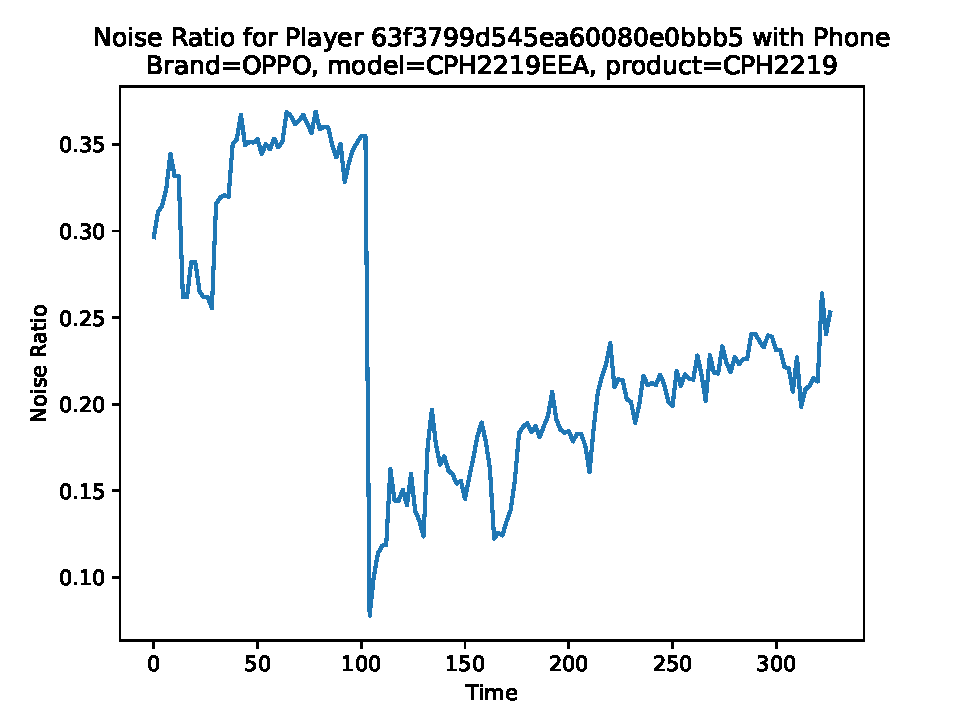
\includegraphics[width=\textwidth]{images/OPPO-CPH2219EEA-123-noiseRatio.pdf}
        \caption{The Noise Ratio during the duration of the game}
        \label{fig:opponoiseratio}
    \end{subfigure}
    
    \caption{This figure shows the catch radius and the noise ratio features using an Oppo F19 phone.
    }
    \label{fig:opponoiseandcatch}
\end{figure}
\begin{figure}
    
    \centering
    \begin{subfigure}[b]{0.48\textwidth}
        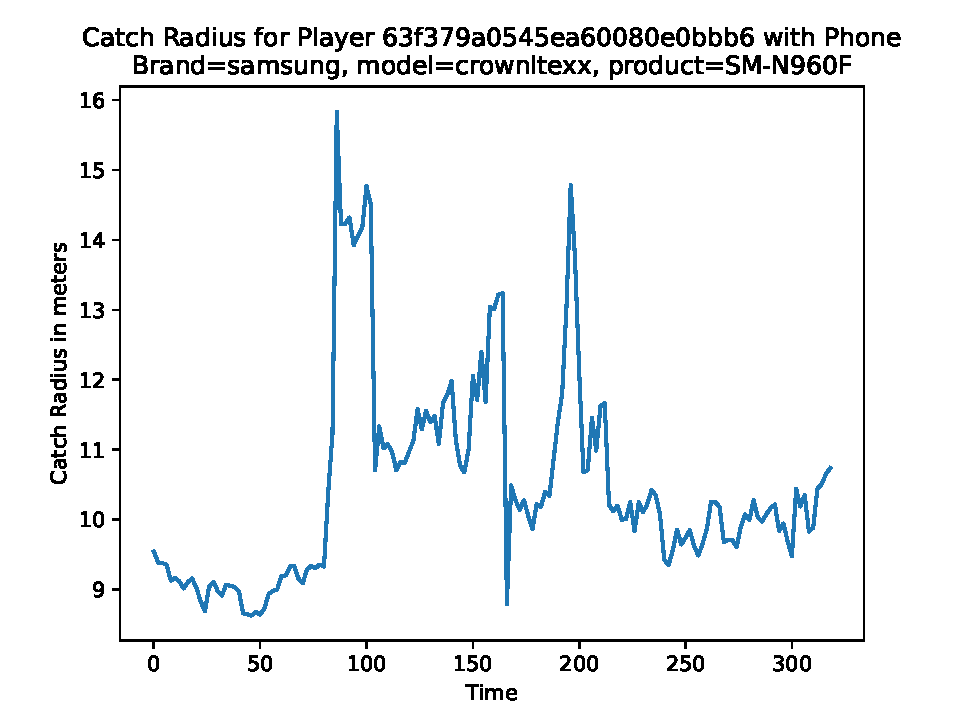
\includegraphics[width=\textwidth]{images/samsung-crownltexx-radius.pdf}
        \caption{The Chase Radius over the duration of the game}
        \label{fig:note9catchradius}
    \end{subfigure}
    ~ %add desired spacing between images, e. g. ~, \quad, \qquad, \hfill etc. 
      %(or a blank line to force the subfigure onto a new line)
    \begin{subfigure}[b]{0.48\textwidth}
        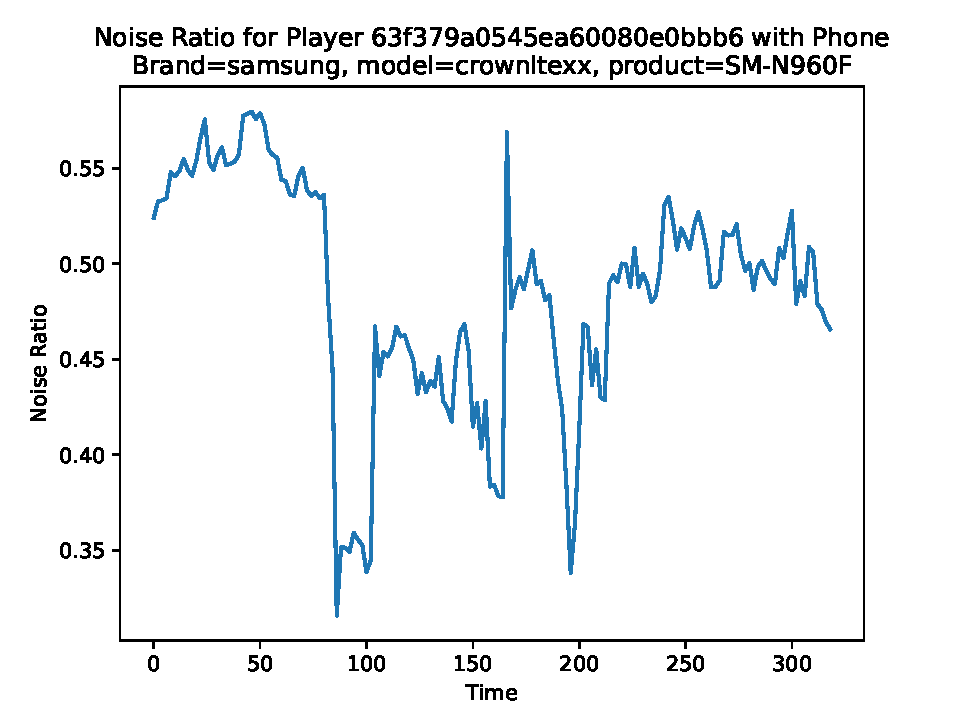
\includegraphics[width=\textwidth]{images/samsung-crownltexx-noiseRatio.pdf}
        \caption{The Noise Ratio during the duration of the game}
        \label{fig:note9noiseratio}
    \end{subfigure}
    
    \caption{This figure shows the catch radius and the noise ratio features using an Samsung Note 9.
    }
    \label{fig:note9noiseandcatch}
\end{figure}
\begin{figure}
    
    \centering
    \begin{subfigure}[b]{0.48\textwidth}
        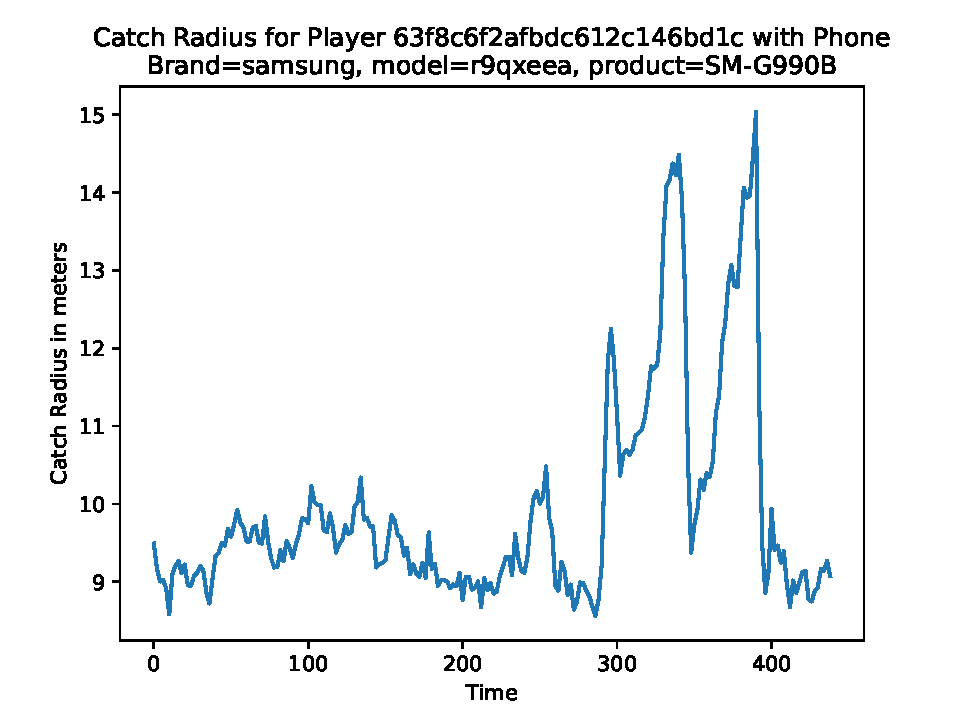
\includegraphics[width=\textwidth]{images/samsung-r9qxeea-radius.pdf}
        \caption{The Chase Radius over the duration of the game}
        \label{fig:s21catchradius}
    \end{subfigure}
    ~ %add desired spacing between images, e. g. ~, \quad, \qquad, \hfill etc. 
      %(or a blank line to force the subfigure onto a new line)
    \begin{subfigure}[b]{0.48\textwidth}
        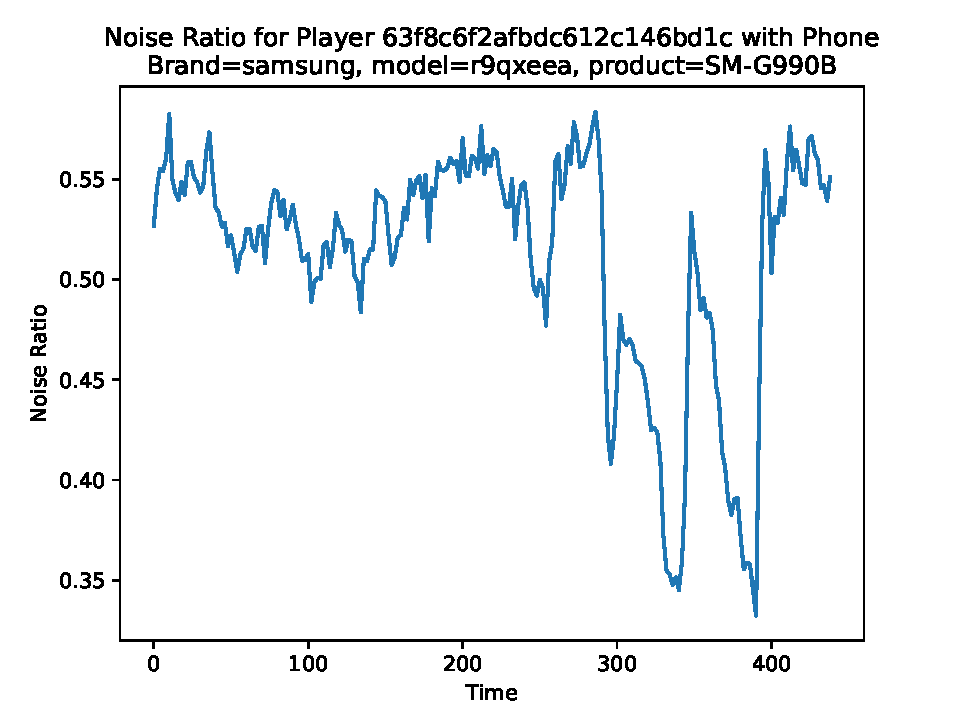
\includegraphics[width=\textwidth]{images/samsung-r9qxeea-noiseRatio.pdf}
        \caption{The Noise Ratio during the duration of the game}
        \label{fig:s21noiseratio}
    \end{subfigure}
    
    \caption{This figure shows the catch radius and the noise ratio features using an Samsung Galaxy S21 FE 5G.
    }
    \label{fig:s21noiseandcatch}
\end{figure}

\chapter{Phase 2 Qualitative Data}

\section{Do you feel that there were any balance issues in the game?}
\label{phase2balance}

\begin{itemize}
    \item Catch radius was too big.
    \item no I think it is balanced
    \item At one point the chaser was able to catch me from far away although I was able to see them. We also switched roles at a random point during a game.
\end{itemize}

\section{Do you have any other comments, feature ideas or feedback?}
\label{phase2generalfeedback}

\begin{itemize}
    \item radius of uncertainty plotted on map as well as catching radius
    \item I really liked the game! It's an interesting concept and made me think about where my GPS signal is strongest and weakest. I also had to use strategy to catch the runner. Unfortunately, I didn't get the chance to use a powerup since I spent most of the game as the chaser. Some possible ideas: - allow some customisability with the pre-game setup, such as choosing how long the game should be - allow the option to extend the game time after it has ended. - make it more clear when the chaser has caught the runner. I didn't realise I had caught the runner until I looked down at my phone and saw that I only had 15 seconds left to run as the runner. Perhaps a modal could flash on screen saying the chaser has been caught and are now swapping roles (maybe even the phone could vibrate).
    \item Overall, it was better experience since the catching mechanic worked much better than before where it didn't work when both players were next to each other. I also found the powerup useful as a runner
\end{itemize}

\chapter{Ethics Checklist}


\includepdf[pages=-]{GPS_Shadows_Ethics_Checklist.pdf}


\end{appendices}

%==================================================================================================================================
%   BIBLIOGRAPHY   

% The bibliography style is abbrvnat
% The bibliography always appears last, after the appendices.

\bibliographystyle{abbrvnat}

\bibliography{l4proj}

\end{document}

